%!TEX TS-program = pdfLaTeX
%!TEX encoding = utf-8
%!TEX spellcheck = en-US

\documentclass[12pt,twoside,openright]{article}

%nœud

%\usepackage{soul}

%\documentclass[a4paper,11pt]{book}
\usepackage[T1]{fontenc}
\usepackage[utf8]{inputenc}
\usepackage[francais]{babel}

\usepackage[usenames,dvipsnames]{color}

\usepackage{lmodern}
%%%%%%%%%%%%%%%%%%%%%%%%%%%%%%%%%%%%%%%%%%%%%%%%%%%%%%%%%
% Source: http://en.wikibooks.org/wiki/LaTeX/Hyperlinks %
%%%%%%%%%%%%%%%%%%%%%%%%%%%%%%%%%%%%%%%%%%%%%%%%%%%%%%%%%
\usepackage{hyperref}
\usepackage{graphicx}
\usepackage{pdfpages}
\usepackage{amsmath}
\usepackage{amssymb}
\usepackage{a4}
\usepackage{indentfirst}
\usepackage{fancyhdr}
\usepackage{varioref}
\usepackage{makeidx}

%\usepackage{biblatex}
\usepackage{mslapa}

\usepackage[normalem]{ulem}

\usepackage{algorithm}
\usepackage{algorithmic}

%% Apalike hyphenation %%%
%\let\oldbibitem=\bibitem
%\renewcommand{\bibitem}[2][]{\oldbibitem[#1]{#2}\newline}

%%% Margins %%%
\voffset -2.54cm
\textheight 24cm
\hoffset -1.3in
\evensidemargin 2.5cm
\oddsidemargin 2.5cm
\textwidth 18cm

% Book's title and subtitle
\title{\textbf{Effective Predictive Control in Fovea-based Scene Decoding} }
% Author
\author{\textsc{Emmanuel Daucé}}%\thanks{\url{www.example.com}}}
\date{}
\makeindex

\begin{document}
	
\maketitle
	
\section{Introduction}

In complement with goal-oriented activity, animal motor control  also relates to the search for sensory clues in order to better interpret its sensory environment and improve action efficacy. This resorts to choosing relevant viewpoints, i.e. selecting body placement and/or sensors orientation in order to capture a sensory signal that should help disambiguate the current scene. It corresponds to selecting views (from a large range of possible views) in order to maximize scene understanding under limited resources constraints. This task is the one considered in this paper (further on called the \emph{sensory scene decoding} task). 

%{\color{magenta} Revue de litterature}

Superior vertebrates oculo-motor activity typically underlies such a decoding task. The important redundancy present in the visual data was exploited by natural selection, ending up in a combination of energy-efficient sensors and resource-saving visuo-motor control, exploiting only little portions of the visual environment to decode the total sensory scene. A salient feature of superior vertebrates visual apparatus is indeed their anosotopic visual sensor, that concentrates  photoreceptors over a small central portion of the retina : the fovea \cite{osterberg1935topography}. Then, by moving the gaze with the eyes, the center of sight is constantly and actively moving around during all waking time. 
This scanning of the visual scene is principally done with high-speed targeted eye movements called saccades \cite{yarbus1967eye}, that sequentially capture local chunks of the visual scene. This makes the oculo-motor activity an essential element of man and animal behavior, underlying most of daily displacements, movements, instrumental and social interactions. 

This scene decoding through action (or ``active perception'') has attracted strong interest in robotics and artificial vision,
%Though ubiquitous in biology, object recognition through saccades is seldom considered in artificial vision. 
 for the important redundancy present in the sensory data allows to envisage energy-efficient  exploring devices  
using  little portions only of the total sensory scene.
%The reasons are many, of which the existence of high-performance sensors that provide millions of pixels at low cost.
The opportunity to neglect large parts of the sensory scene should mainly be considered when the energy is scarce, as it is the case for drones and robots. 
It is also relevant in computer vision, where mega-pixel images appeals for selective convolutions, in order to avoid unnecessary matrix products. 
The example of animal vision thus encourages a more parsimonious approach to robotic and computer vision, \emph{including the control of the sensory flow}. 
%A computer vision program should for instance look back from past experience to see which viewpoint to use to provide the most useful information about a scene. 
Optimizing the sensor displacements across time may then be a part of robotic control, in combination with goal-oriented operations. 

%itself, with critical or useful information only present in 

 %Though taking a large part in brain activity, the principles underlying those visually guided movements are still a subject of debate in neurosciences.
%The most documented case of active perception is gaze orientation, primarily studied in both man and animal \cite{yarbus1967eye,robinson1968eye}. A nice review of principal promises of \emph{animate} vision against passive vision  is presented in \cite{ballard1991animate},  in relation with eye-hand coordination in computer vision.
%
%, {\color{magenta} following an approximate exponential decrease of resolution from the center to the periphery [REF?]}. 
 %\footnote{in contrast with animals retina whose actual design relies on a long optimization process under severe resource constraints.}.
%Increasingly powerful computing devices are then assigned to compute in parallel those millions of pixels to perform recognition, consuming resources in a brute-force fashion. 


%A salient aspect of animal vision is the use of \emph{active} sensing devices, capable of moving around under some degrees of freedom in order to choose a particular viewpoint. The existence of a set of possible sensor movements calls for the development of specific algorithms that should \emph{solve the viewpoint selection problem}. 

\paragraph{}
Changing the viewpoint can be seen as a way to leverage ambiguities present in the current visual field. In \cite{aloimonos1988active}, the authors show that some ill-posed object recognition problems become well-posed as soon as several views on the  same object are considered. A more general perspective is developed in \cite{bajcsy1988active}, with a first attempt to interpret active vision in the terms of sequential Bayesian estimation:
\begin{quote}
	\emph{The problem  of Active Sensing can be stated as a problem of controlling strategies 
		applied to the data acquisition process which will depend on the current state 
		of the data interpretation and  the  goal  or the  task of  the  process.}
\end{quote}
thus providing a roadmap for the development of active vision and sensory systems.

Work on central vision control is quite scarce until the late 2000's.
On the machine learning side, an example of fovea-based visuo-motor control was  addressed in \cite{schmidhuber1991learning}, with a direct policy learning from gradient descent by using BPTT through a pre-processed forward model. 
On the biological  side, early models from the late nineties  consider the case of fovea-based image encoding, ending up in the simplified ``pyramidal'' focal image encoding model \cite{kortum1996implementation}. Active vision models were however largely dominated by the \emph{salience} models \cite{itti2000saliency,itti2001computational,itti2005bayesian}, that are known to provide among the best fit with the preferred fixation zones observed in humans. 
Motor control were however generally bypassed in that case, putting the focus on characterizing the attractiveness of fixation zones rather that explicitating 
%a sequential step-by-step 
the image decoding process through changing fixation point.
%Despite their strong explanatory power, they generally bypass central/foveal vision aspects. 
Combined with a focal pyramidal image encoding, the salience approach  still provides effective outcome in image and video compression  \cite{wang2003foveation,guo2010novel}.


The salience approach to active vision is generally referred as a ``bottom-up'' approach, for only low-level aspects of the images are considered in the decoding process. In contrast, scene interpretation and active object search in images is generally referred as the ``top-down'' approach, for ``high level'' assumption are made over the actual content of the image. 
%The idea of viewpoints selection turns out to consider beforehand the pixels that need to be processed to achieve the scene decoding. 

Two parallel research tracks adopted and refined this very idea over the last twenty years.
On the one side, human visual search modeling considers action as  \emph{sampling} over an underlying (covert) sensory scene obeying to a mixture generative model. 
%The general principle is that of choosing the sample that is the most {\color{blue} informative} \emph{in expectation}. 
%Then appropriate viewpoints should be selected to maximize the \emph{decoding accuracy}, that resorts to refine the beliefs about the underlying scene to reduce the posterior entropy. 
Stemming from \cite{bajcsy1988active}'s intuition, a \emph{predictive} approach to perception-driven control was originally developed in \cite{najemnik2005optimal} to the case of visual search.
It globally complies with the predictive coding framework \cite{rao1999predictive} with the current posterior estimate used to anticipate future sensations. 
%, later on refined in a \emph{posterior entropy} minimization principle \cite{najemnik2009simple}.
%Follow-up work of \cite{butko2010infomax} provide a comprehensive overview of a foveated POMDP-based active vision, with examples of visual search in static images using a bank of pre-processed features detectors. 
Here, appropriate samples should be selected that maximize the expected \emph{decoding accuracy}, that resorts to reduce the number of possible interpretations of the underlying scene, i.e. reduce the expected posterior entropy (see \cite{najemnik2005optimal,najemnik2009simple,butko2010infomax,friston2012perceptions}).
More generally, the idea of having many (i.e. a mixture of) models to identify a scene complies with the weak classifiers evidence accumulation principle developed in computer vision (see \cite{viola2003fast} and sequels). It also generalizes to the multi-view selection in object search and scene recognition \cite{potthast2016active}.

A second research track insists on the formal contribution of action in the \emph{encoding} of the (future) sensory field. This resorts to consider action as a \emph{code} that is later on revealed (decoded) by sensing the effect of action at the visual field \cite{klyubin2005empowerment,tishby2011information}. As such it may be optimized so as to maximize the code expressiveness, allowing to improve both the policy and the data model in the course of learning \cite{schmidhuber2007simple,mohamed2015variational,houthooft2016vime}.


This interestingly conducts to develop different objective functions that do not appear mutually compatible in a first place.
The sampling efficacy objective encourages actions that provide a consistent belief update, measured at the log likelihood of the data after sampling. This implies to avoid surprising data and prefer actions that provide a sensory input that is consistent with the initial guess \cite{friston2010free}. This  approach may be referred as the ``conservation-based'' approach to action selection.  
In contrast, the encoding efficacy objective encourages actions that provide informationally-rich content, which is formally defined as the information gain provided by improving the prediction after taking action, also known as the ``surprise'' \cite{itti2005bayesian}. This second approach may be referred as the ``innovation-based'' approach to action selection. 

The principle of this paper is trying to reconcile both views by considering action as both a sampling and a code, through a mere bijection between the motor command and the actuator state, also known as the ``end-effector control''. The current observation becomes the decoding of a \emph{mixed code}  
made of a controlled code (i.e. the actuator state) and an uncontrolled one (i.e. the rest of the environment). This idea is first mathematically developed in section \ref{sec:material}, providing a way to interpret the different objective functions found in the literature under a single master equation referred as the \emph{Compression Improvement} \cite{schmidhuber2007simple}. 
Then a fovea-based implementation is proposed in section \ref{sec:results}, allowing to compare in detail the different options in a single setup, and propose new avenues toward more parsimonious scene decoding through computationally-effective model-based prediction.

\section{Material and methods} \label{sec:material}

We consider here a \emph{scene decoding task} where an agent has to estimate its environment state, here called the ``sensory scene'' from sensory samples. The visual scene is organized in objects (or objects parts), whose presence and position is continuously checked by visual inspection. 
Then, decoding a visual scene through saccades consists in identifying the ensemble through the sequential foveation of parts of the scene only. 

\subsection{A ``Three-Party'' generative model}\label{sec:three-party}

A ``viewpoint emitter'' $\boldsymbol{u}$ is here interpreted as both the realization of a \emph{sampling} (of an underlying generative model), and as a \emph{code} that participates in generating the incoming sensory data.




%The combination of  (\ref{eq:process}) and (\ref{eq:measure}) is said a \emph{generative process} that is 

%{\color{magenta} probabilistic framework : the changes that take place in the physical world described by  = model.}
%Given an initial state $\boldsymbol{z}_0$, the next state $\boldsymbol{z}$ rests on the conditional distribution   and the 



\subsubsection{One scene, many views}

%\subsubsection{Generic feedback control framework and generative process}
%\paragraph{Generative process}
A feedback control framework is composed of an actor and an environment. The actor and the environment interact according to a feedback loop. 
The actor can act on the environment through its effectors, and sense the state of the environment through its sensors. 
The state of the environment as well as the state of the agent can change over time. The state of the environment is described by a state vector $\boldsymbol{s} \in \mathcal{S}$.
%In a Markovian framework, the state $\boldsymbol{s}$ in which the physical system is found at present depend both on its previous state (say $\boldsymbol{s}_0$) and on a preceding motor command $\boldsymbol{a}$ 
%The transition from $\boldsymbol{s}_0$ to $\boldsymbol{s}$ is reflected in a \emph{transition function} that embodies the deterministic and non-deterministic effects of the command $\boldsymbol{a}$ in a conditional probability distribution:  
%\begin{align}
%\boldsymbol{s} \sim \text{Pr}(S|\boldsymbol{a},\boldsymbol{s}_0) \label{eq:process}
%\end{align}
%implemented with a probability density function 
%$p_\text{\sc trans}(\boldsymbol{s}|\boldsymbol{a},\boldsymbol{s}_0)$.
The signal $\boldsymbol{x}$ that is measured on the sensors is called the \emph{sensory field}. It is interpreted as a measure made by the sensors, that is causally related to the current state $\boldsymbol{s}$. 
The dependence between $\boldsymbol{s}$ and $\boldsymbol{x}$ is reflected in a conditional probability distribution:
%\begin{align}
%\boldsymbol{x} \sim \text{Pr}(X|\boldsymbol{s})\label{eq:measure}
%\end{align}
%implemented with a probability density function 
$p(\boldsymbol{x}|\boldsymbol{s})$, that is said the \emph{generative model}, i.e. the cause of the sensory field..
We considers here an organization a the visual scene in objects (or object parts), whose presence and position is continuously checked by motor inspection. 
We moreover suppose that a generative model $p$ is given to the agent.

%Put formally, exploring a visual scene through saccades consists in identifying objects in space through the foveation of parts of the scene only. 
Put mathematically, the cause $\boldsymbol{s}$ of the current visual field $\boldsymbol{x}$ is both the object identity $\boldsymbol{o}$, its position in the peripersonal space $\boldsymbol{y}$, and the current visual orientation $\boldsymbol{u}$, i.e. $\boldsymbol{s} = (\boldsymbol{y},\boldsymbol{o},\boldsymbol{u})$ and $\boldsymbol{x} \sim P(X|\boldsymbol{y},\boldsymbol{o},\boldsymbol{u})$, each variable counting for a distinct degree of freedom. This description of the sensory emitter as a three degrees of freedom construct is called here the ``\emph{Three-Party}'' model.

We propose here to split the generative process in two parts, namely the controlled generative process and the uncontrolled generative process. 
This separation 
is consistent with the ``hidden state''/``hidden control'' distinction stated in \cite{friston2012perceptions}.
The controlled emitter is $\boldsymbol{u}$ while the uncontrolled emitter is  $(\boldsymbol{y}, \boldsymbol{o})$. 
For greater simplicity, $(\boldsymbol{y},\boldsymbol{o})$ is here reduced to a single variable $\boldsymbol{z} = (\boldsymbol{y}, \boldsymbol{o})$, 
so that the generic uncontrolled variable $\boldsymbol{z}$ may report for every possible composition of object identity in space (or more generally every composition of a pose and an identity).
%for we more specifically put the focus here on the controller setup.% and the generative process   $o \in \mathcal{O}$, position $x \in \mathcal{X}$ and $u \in \mathcal{U}$. 
The controlled emitter $\boldsymbol{u}$ refers to the state of a motor apparatus, e.g. to the spatial distribution of the different mobile segments of an articulated body. The uncontrolled latent emitter $\boldsymbol{z}$  refers to the remaining part of the physical world, i.e. the ``environment''. 

This restricted setup, that separates a body and an environment in the form of two parallel processes,  provides a substantial simplification to the estimation problem at stake: 
\paragraph{(i) Emitters independence}
A first assumption is that two emitters are independent, i.e. $p(\boldsymbol{z}, \boldsymbol{u}) = p(\boldsymbol{z})p(\boldsymbol{u})$ so that:
\begin{align}
(\boldsymbol{z},\boldsymbol{u}) \sim \text{Pr}(Z,U|\boldsymbol{a}, \boldsymbol{z}_0, \boldsymbol{u}_0) = \text{Pr}(Z|\boldsymbol{a}, \boldsymbol{z}_0, \boldsymbol{u}_0) \text{Pr}(U|\boldsymbol{a}, \boldsymbol{z}_0, \boldsymbol{u}_0)\nonumber
\end{align}
	
\paragraph{(ii) End-effector control}
An additional assumption is that the controlled generative process is relatively ``fast'' in comparison with the uncontrolled one
(for, e.g, saccades can be realized in a 100-200 ms interval). 
In consequence we assimilate the motor command $\boldsymbol{a}$ with a setpoint (or posture) $\boldsymbol{u}$ in the actuator space, that is supposed to be reached 
at short notice by the motor apparatus once the command is emitted, under classical stability/controllability constraints.
This entails that, consistently with the `end-effector'' ballistic control setup \cite{mussa2004neural},  \emph{$\boldsymbol{u}$ is independent from $\boldsymbol{u}_0$},
i.e.:
\begin{align*}
\boldsymbol{u}\sim\text{Pr}(U|\boldsymbol{a})
\end{align*}

The motor command $\boldsymbol{a}$ then corresponds to the desired end-orientation of the sensor,
% here considered as a setpoint on the actuators space, 
either expressed in actuators or endpoint coordinates (with hardware-implemented detailed effector response function).  
Under that perspective, the effector acts on the sensors position and orientation so as to achieve a certain perspective (or view) over the external scene, and the controlled emitter $\boldsymbol{u}$ is now called a \emph{viewpoint}. 

\paragraph{(iii) Uncontrolled environment}
The third important assumption is that the motor command $\boldsymbol{a}$ \emph{is not expected to affect on the uncontrolled latent emitter $\boldsymbol{z}$}, i.e.
\begin{align*}
\boldsymbol{z} \sim \text{Pr}(Z|\boldsymbol{z}_0)
\end{align*}
so that $\boldsymbol{z}$ should depend only on the external dynamics (the external ``uncontrolled'' process).

\paragraph{(iv) Static assumption}
Under a scene decoding  task, %where the motor command $\boldsymbol{u}$ refers to the orientation of a sensor, 
it is rather common to consider the environment as ``static'' \cite{butko2010infomax}. This fourth assumption means, in short, that:
$$\text{Pr}(Z|\boldsymbol{z}_0) = \delta(Z, \boldsymbol{z}_0)$$ 
with $\delta$ the Knonecker symbol. 
The uncontrolled latent emitter $\boldsymbol{z}$ is thus expected to capture all relevant information about the current scene, while remaining invariant throughout the decoding process.


At last, the measure $\boldsymbol{x}$ may rely on both emitters $\boldsymbol{z}$ and $\boldsymbol{u}$, i.e. 
\begin{align}
\boldsymbol{x} \sim \text{Pr}(X|\boldsymbol{z}, \boldsymbol{u})
\label{eq:gen}
\end{align} 
Each measure $\boldsymbol{x}$ is generated from a mixed emitter $(\boldsymbol{z}, \boldsymbol{u})$, with $\boldsymbol{u}$ the controlled part of the emitter and  $\boldsymbol{z}$ the uncontrolled part. Note that $\boldsymbol{z}$ is said the latent state out of habit, though both $\boldsymbol{u}$ and $\boldsymbol{z}$ contribute to the generation of $\boldsymbol{x}$.

For notational simplicity, we absorb here the execution noise \cite{van2004role} in the measure process, i.e.:
$\boldsymbol{x} \sim \text{Pr}(X|\boldsymbol{z}, U)\text{Pr}(U|\boldsymbol{a})$.
Then, by notational abuse, we assimilate in the rest of the paper  $\boldsymbol{u}$ (the controlled emitter) with $\boldsymbol{a}$ (the motor command), so that 
a single variable $\boldsymbol{u} \equiv \boldsymbol{a}$ should be used for both. %We also call the uncontrolled latent emitter $\boldsymbol{z}$ the \emph{latent state} for simplicity.
Each different $\boldsymbol{u}$ is thus both interpreted as a
motor command and as a code. As a motor command, it is controllable, i.e. determined by a controller. As a code, it monitors the generation of the sensory field (decoding), in combination with the latent state $\boldsymbol{z}$. 


%with $p(X|\boldsymbol{z}, \boldsymbol{u})$ the forward model,  conditioned on both $\boldsymbol{z}$ and $\boldsymbol{u}$, so that the latent state space (the cause of the visual field) now decomposes in an uncontrolled emitter $\boldsymbol{z}$ and an explicit motor command $\boldsymbol{u}$, and $p(Z)$ the \emph{prior}. 
 %, so that $p(X,Z,U) = p(X|Z, U) p(X, U)$. 



%The generative model may finally write:
%\begin{align}
%p(X, Z, U) = p_\text{\sc meas}(X| Z, U)p_\text{\sc prior}(Z) p_\text{\sc prior}(U)
%\end{align}
%It should be noted that the dependencies between the three variables can moreover be symetrically decomposed in the form of three conditional models, i.e. :
%\begin{align}
%p(X, Z, U) &= p(X| Z, U) p(Z)p(U)\nonumber\\ 
%&= p(Z| X, U)p(X) p(U)\nonumber\\
%&= p(U|X, Z)p(X) p(Z)\label{eq:three-party}
%\end{align}
%comprising a \emph{forward model} $p(X|\boldsymbol{z}, \boldsymbol{u})$ 
%conditioned on both $\boldsymbol{z}$ and $\boldsymbol{u}$,  an \emph{inverse model} $p(Z|\boldsymbol{x}, \boldsymbol{u})$  conditioned on both on  $\boldsymbol{x}$ and $\boldsymbol{u}$ and an ``\emph{inverse controller}'' $p(U|\boldsymbol{x}, \boldsymbol{z})$ conditioned on both on  $\boldsymbol{x}$ and $\boldsymbol{z}$. This boils down to implementing three variants of a two \emph{degrees of freedom} generative model. 



%

%The generative distribution becomes $p(\boldsymbol{x}, \boldsymbol{z}, \boldsymbol{u})$ so that activating the motor effectors updates the state of the plant as well as its visual sensory outcome. In comparison,  i.e.: %changing the state of an external (uncontrolled) emitter would also modify the visual sensory outcome. The command $u$ here participates in a feedback loop that in return updates the visual stream.
% This generative model is written:
%$$p(X, Z, U) = p_\text{\sc meas}(X| Z, U)p_\text{\sc prior}(Z, U)$$
%It can further on be simplified by considering that the measure captures all the relevant dependencies, i.e. that $X$ is conditionally dependent on the $(U,Z)$ couple, but independent from $U$ alone and independent from $Z$ alone, while $U$ and $Z$ are also mutually independent, i.e.:

Finally, both $\boldsymbol{x}$ (the view) and $\boldsymbol{z}$ (the \emph{latent state}) are the realization of a generative model parametrized by $\boldsymbol{u}$, i.e.
\begin{align}
\boldsymbol{x}, \boldsymbol{z} | \boldsymbol{u} \sim \text{Pr}(X|Z, \boldsymbol{u}), \text{Pr}(Z) \label{eq:generative}
\end{align}  
with $p(Z)$ the \emph{prior}, and each different motor command $\boldsymbol{u}$ providing a different sample over the same underlying distribution. Under that prospect, the action $\boldsymbol{u}$ is interpreted as a \emph{sampling} operation.

\subsubsection{Sequential Bayesian inference}\label{sec:seq-bayes}


With a generative model comes the possibility to \emph{infer} the latent state of the physical system 
%$\boldsymbol{s}$ from the sensory field $\boldsymbol{x}$, the previous state $\boldsymbol{s}_0$ and the motor command $\boldsymbol{a}$ 
using Bayes rule:
\begin{align}
\text{Pr}(Z|\boldsymbol{x},\boldsymbol{u})
= \frac{\text{Pr}(\boldsymbol{x}|Z, \boldsymbol{u}) \text{Pr}(Z)}
{\text{Pr}(\boldsymbol{x}|\boldsymbol{u})}\label{eq:post-Pr}
%&= \frac{\text{Pr}(X|Z,\boldsymbol{u}) \text{Pr}(Z|\boldsymbol{u},\boldsymbol{z}_0)}{\sum_{\boldsymbol{z}'}\text{Pr}(X|\boldsymbol{z}',\boldsymbol{u}) \text{Pr}(\boldsymbol{z}'|\boldsymbol{u},\boldsymbol{z}_0)}\label{eq:post}
\end{align}
with $\text{Pr}(Z|\boldsymbol{x},\boldsymbol{u})$ the \emph{posterior} probability (a distribution over the latent states) whose order 2 moment informs on the estimation accuracy : the narrower the distribution, the more accurate the latent state prediction. 

The chaining of the posterior to the role of the prior in the next inference step is a classical property of sequential Bayesian inference \cite{wald1945sequential}.
When generalized to many observations: $(\boldsymbol{x}|\boldsymbol{u}), (\boldsymbol{x}'|\boldsymbol{u}')$, ..., $(\boldsymbol{x}^{(n)}|\boldsymbol{u}^{(n)})$, the final posterior $q^{(n)}(Z)$ writes:
\begin{align}
q^{(n)}(Z) \propto p(\boldsymbol{x}|Z,\boldsymbol{u}) p(\boldsymbol{x}'|Z,\boldsymbol{u}') ... p(\boldsymbol{x}^{(n)}|Z,\boldsymbol{u}^{(n)}) \label{eq:accum}
\end{align}
which allow to approach the latent state $\boldsymbol{z}$ from many samples of (\ref{eq:gen}), each sample providing more evidence. 
It is noteworthy that the $\boldsymbol{u}$'s and $\boldsymbol{x}$'s do not need to be stored in the process. At step $n$, only $q^{(n-1)}$ (the current ``belief'') needs to be memorized to estimate $q^{(n)}$, i.e. 
\begin{align} 
q^{(n)}(Z) \propto p(\boldsymbol{x}^{(n)}|Z,\boldsymbol{u}^{(n)}) \times q^{(n-1)}(Z) \label{eq:accum-post}
\end{align}





%$\boldsymbol{z}$ $\boldsymbol{s} = (\boldsymbol{z}, \boldsymbol{u})$. 

\subsection{Perception-driven control}\label{sec:perception-driven-control}

In our ``three-party'' framework, 
%called here the ``three party'' generative setup, 
saccadic exploration finally means to define a sequence of visuo-motor commands $\boldsymbol{u}$, $\boldsymbol{u}'$, $\boldsymbol{u}''$, ... This sequence should ultimately provide a final estimate $\hat{p}(\boldsymbol{z})$ with a single cause $\hat{\boldsymbol{z}}$ dominating the other ones, allowing the system to reach a final decision. This is the \emph{scene decoding} task we analyze next.




%Here the role of the controller is not to achieve a goal-oriented task, but to render the estimation of the latent state more accurate. The controller is said \emph{perception-driven}. 
%The design of such a controller is not straightforward. 
%On contrary to classical control, there is not definite setpoint $\boldsymbol{z}^*$ to which the controller is supposed to drive the external process (through model inversion for instance). 
\subsubsection{Active sampling}

Consider an agent having to estimate its environment state $\boldsymbol{z}$ from sampling it from different viewpoints. We here suppose that a generative model  is given to the agent. 
Depending on  the current viewpoint $\boldsymbol{u}$, a different view $\boldsymbol{x}$ is observed at the sensors. So, each different command $\boldsymbol{u}$ provokes a different observation, and thus a different 
estimation of the latent state. It is thus worth to question what is the optimal choice for $\boldsymbol{u}$ in order to maximize the accuracy of the posterior estimate?
That turns  to minimize the number of samples so as to provide an accurate estimate. This approach to inference is called \emph{active sampling} \cite{friston2012perceptions}, for the choice of $\boldsymbol{u}$ determines the sensory sample $\boldsymbol{x}$ that is observed, conditioning the final posterior estimate.

A baseline sampling strategy is to choose $\boldsymbol{u}$ at random and condition the posterior  estimate on this random action. 
More elaborate strategies consider the past observations
%$\{\boldsymbol{u}^{(1:n-1)}, \boldsymbol{x}^{(1:n-1)}\}$ 
to choose the most promising action $\hat{\boldsymbol{u}}$. %We have seen in  \ref{sec:perception-driven-control} that, under a Markov assumption, the memory of the past context
%at step $n$ .  
%We have seen in  \ref{sec:perception-driven-control} that, under a Markov assumption, the memory of the past context
%at step $n$ can be absorbed in single posterior distribution $q^{(n-1)}$.  
The knowledge about past observations being here absorbed in single posterior distribution $q^{(n-1)}$, the problem turns out to design  a \emph{controller} $C$ which, given a context $q^{(n-1)}$, sets up an action $\hat{\boldsymbol{u}} = C(q^{(n-1)})$. Here the role of the controller is not to achieve a goal-oriented task, but to render the estimation of the latent state more accurate. The controller is said \emph{perception-driven}. 

The design of such a controller is not straightforward. On contrary to classical control, there is not definite setpoint $\boldsymbol{z}^*$ to which the controller is supposed to drive the external process (through model inversion for instance). By design, the actual latent state $\boldsymbol{z}$ is not visible as such and can not be compared to the inferred posterior. In order to estimate how good a motor command is, one needs to provide an estimate of the value-of-action (regarding scene understanding). There is currently no consensus about what a good value is regarding the scene decoding task. 

A general strategy is thus to establish a \emph{objective function} $f$ (resp. a loss $\ell$) that conveys a quantitative estimation of the action's contribution to the inference accuracy (resp. imprecision). Once the objective function established, a simple control strategy is to choose the action that maximizes the objective (resp. minimizes the loss), i.e.:
\begin{align}
\hat{\boldsymbol{u}} = \underset{\boldsymbol{u}\in\mathcal{U}}{\text{ argmin }}  \ell(\boldsymbol{u})\left/ \underset{\boldsymbol{u}\in\mathcal{U}}{\text{ argmax }}  f(\boldsymbol{u})\right.
\end{align}
Many such objective functions are proposed in the literature. They are generally referred as an \emph{intrinsic} motivation \cite{oudeyer2008can} by contrast with the \emph{extrinsic} motivation that relates to the classical rewards in reinforcement learning \cite{sutton1998reinforcement}. Several intrinsic reward candidates can be developed in the scene decoding context.
%We propose here a tour of the most common intrinsic value estimators and reformulate them under the scene decoding setup \footnote{Note the estimators provided here are compatible with the POMDP setup, but restrained to the ``three-party'' case --~see eq.~(\ref{eq:three-party})~-- for mathematic simplicity.}, and try to evaluate the pros and cons of the different approaches.
%, and end up with new objective formulation called the \emph{encoding accuracy}. 


\subsubsection{Predictive control}\label{sec:infomax}


The predictive approach to perception-driven control was originally developed by \cite{najemnik2005optimal} to the case of visual search (finding a target feature in an image, i.e. the ``find Waldo'' task).
Considering a  probabilistic generative model $p(X,Z,U)$, like the one described in section \ref{sec:three-party}, the predictive approach relies on predicting an \emph{accuracy} measure $A(\boldsymbol{x}, \boldsymbol{u}, q^{(n-1)})$ to choose action. 
The accuracy tells how good the model is at predicting $\boldsymbol{z}$ (here the target position) when viewing $\boldsymbol{x}$ at position $\boldsymbol{u}$,
knowing $q^{(n-1)}$ (the estimated posterior at step $n-1$).

If the agent has to choose an action $\boldsymbol{u} \in \mathcal{U}$, knowing only $q^{(n-1)}$, the \emph{predicted} accuracy attached to $\boldsymbol{u}$ is:
\begin{align*}
\bar{A}(\boldsymbol{u}; q^{(n-1)})
&= \mathbb{E}_{\boldsymbol{z} \sim q^{(n-1)}(Z), \boldsymbol{x} \sim p(X|\boldsymbol{z}, \boldsymbol{u})}\left[A(X, \boldsymbol{u}; q^{(n-1)})\right]  \\
&= \sum_{z\in\mathcal{Z}} q^{(n-1)}(\boldsymbol{z}) \int_{\mathcal{X}}  A(\boldsymbol{x}, \boldsymbol{u}; q^{(n-1)}) p(\boldsymbol{x}) d\boldsymbol{x}  
\end{align*}
and the optimal action to choose is:
\begin{align}
\hat{\boldsymbol{u}} = \underset{\boldsymbol{u} \in \mathcal{U}}{\text{ argmax }} \bar{A}(\boldsymbol{u}; q^{(n-1)})\label{eq:predictive-policy}
\end{align} 
It must be noted that in order to render the computation tractable, a \emph{sampling} approach is generally used to estimate the predicted accuracy, i.e. $\mathbb{E}_p[f(\boldsymbol{x})] \simeq f(\tilde{\boldsymbol{x}})$, with $\tilde{\boldsymbol{x}}\sim p(\boldsymbol{x})$.

The accuracy measure used in the original paper was an ad-hoc one \cite{najemnik2005optimal}, but turned out to be consistent with minimizing the \emph{posterior entropy} \cite{najemnik2009simple}, i.e.:
$$A(\boldsymbol{x}, \boldsymbol{u}; q^{(n-1)}) = -H(q^{(n)}) = \sum_{z \in \mathcal{Z}} q^{(n)}(\boldsymbol{z}) \log q^{(n)}(\boldsymbol{z})$$
with: $q^{(n)}(\boldsymbol{z}) \propto p(\boldsymbol{x|\boldsymbol{z}, \boldsymbol{u}})q^{(n-1)}(\boldsymbol{z}) $
so that:
$$\hat{\boldsymbol{u}} = \underset{\boldsymbol{u} \in \mathcal{U}}{\text{ argmin }} \mathbb{E}_{q^{(n-1)},p}\left[H(q^{(n)})\right] $$ 
which makes sense for a low entropy of the posterior is expected when the estimated posterior accuracy is high.

%This approach to optimal visual sampling was further on linked to an ``Infomax'' principle in \cite{butko2010infomax} and shown efficient in artificial visual search using policy gradient \cite{williams1992simple} to learn the controller. 


This approach to optimal visual sampling was further on linked to an ``Infomax'' principle in \cite{butko2010infomax} 
%and shown efficient in artificial visual search using policy gradient \cite{williams1992simple} to learn the controller, with 
taking
\begin{align}A(\boldsymbol{x}, \boldsymbol{u}; q^{(n-1)}) \equiv I(Z; \boldsymbol{x}|\boldsymbol{u}; q^{(n-1)})
= H(Z|q^{(n-1)}) - H(Z|\boldsymbol{x}, \boldsymbol{u}; q^{(n-1)})
\label{eq:infomax}
\end{align}
with  $H(Z|q^{(n-1)}) \equiv H(q^{(n-1)})$ and $H(Z|\boldsymbol{x}, \boldsymbol{u}, q^{(n-1)}) \equiv H(q^{(n)})$.
The Infomax (or posterior entropy minimization) approach generally makes sense for it implicitly relies on the chaining from $q^{(n-1)}$ to $q^{(n)}$, that considers that if $p(\boldsymbol{x}|Z, \boldsymbol{u})$ is consistent with $q^{(n-1)}(Z)$, then the issued posterior entropy should be lower than if $p(\boldsymbol{x}|Z, \boldsymbol{u})$ is at odd with $q^{(n-1)}(Z)$. The model is expected to choose the action that may confirm the initial assumption, though there is no comparison between $q^{(n-1)}$ and $q^{(n)}$.
It is thus potentially vulnerable to model outliers with $q^{(n)}$ having both a low entropy and being inconsistent with $q^{(n-1)}$.





\subsubsection{Innovation-based control}\label{sec:saliency}

%In contrast, the ``top-down'' approach considers viewpoint change as a prototype of action selection in the brain. 
%Interestingly, very similar concepts and modelling tools can be used in both the bottom-up and top-down approaches. 
%The main difference is that the top-down approach implements a sequential Bayesian accumulation procedure (see eq~\ref{eq:accum}) to reflect belief change and viewpoint selection over time. $q^{(n-1)}$ is now the current belief about that latent state, that plays the role of the current ``model''. Then, every viewpoint $\boldsymbol{u}$ may reveal more or less consistent with $q^{(n-1)}$. 
%The baseline consistency between  $\boldsymbol{u}$ and $q^{(n-1)}$ is provided by~:
%$$v() = \text{KL}(q^{(n)}||q^{(n-1)})$$
%with $q^{(n)}$ updated according to eq.~(\ref{eq:accum-post}).

%Let this consistency be noted $v(\boldsymbol{x}, \boldsymbol{u}, q^{(n-1)})$. Considering that:
%\begin{enumerate}
%	\item $v(\boldsymbol{x}, \boldsymbol{u}, q^{(n-1)})=q^{(n)}(\hat{\boldsymbol{z}})$
%	with $\hat{\boldsymbol{z}} = \underset{\boldsymbol{z}}{\text{argmax }}q^{(n)}(\boldsymbol{z})$ 
%	the ``accuracy'' of posterior in .
%	\item $v(\boldsymbol{x}, \boldsymbol{u}, q^{(n-1)})=-H(q^{(n)})$
%	with $H(q^{(n)}) = - \sum_z q^{(n)}(\boldsymbol{z})\log q^{(n)}(\boldsymbol{z})$
%	the entropy of the posterior in \cite{najemnik2009simple,butko2010infomax,friston2012perceptions}
%\end{enumerate} 



Another quantity of interest is the so-called \emph{Bayesian surprise} or \emph{Salience} \cite{itti2005bayesian} defined as the Kullback-Leibler divergence  between an actual view $\boldsymbol{x}$ and a model $\boldsymbol{z}$. In the original ``bottom-up'' setup, only local statistics $q$ are formed over small image patches of a given image, with $\boldsymbol{u}$ the index of a patch and $p(\boldsymbol{z}|\boldsymbol{x},\boldsymbol{u})$ the features inferred from the data actually observed at $\boldsymbol{u}$. For each patch $\boldsymbol{u}$, the Salience of the actual view $\boldsymbol{x}$ given the model is:
$$ S(\boldsymbol{x},\boldsymbol{u}) = \text{KL}(p(Z| \boldsymbol{x}, \boldsymbol{u})||p(Z))$$
which is a measure of the \emph{in}consistency between a (viewpoint independent)  model $p$ and the data. A high salience reflects a strong inconsistency with the model, while a low salience reflects a strong consistency with the model.

Generalized to the sequential setup, the saliency measure becomes:
\begin{align} S(\boldsymbol{x}^{(n)},\boldsymbol{u}^{(n)}; q^{(n-1)}) = \text{KL}(q^{(n)}(Z)||q^{(n-1)}(Z))\label{eq:saliency}
\end{align}
with $q^{(n-1)}$ considered as the data model and $q^{(n)}$ the posterior estimated at $(\boldsymbol{x}^{(n)},\boldsymbol{u}^{(n)})$.
%It interestingly shares a formal similarity with the second term of the variational Free Energy (see eq.\ref{eq:FEP-uxun}). 

According to Itti and Baldi, the regions that have a high Bayesian surprise are the ones that attract the sight the most. The calculation of $S(\boldsymbol{x}, \boldsymbol{z}| \boldsymbol{u})$ at each location $\boldsymbol{u}$ forms a \emph{saliency map} that is then considered as a prediction of where the sight will most likely be attracted (high values most probably attract the sight, low values less probably do). 
In a sequential setup, a corresponding predictive policy would be:
$$ \hat{\boldsymbol{u}} = \underset{\boldsymbol{u} \in \mathcal{U}}{\text{ argmax }} \mathbb{E}_{\boldsymbol{z} \sim q^{(n-1)}(Z), \boldsymbol{x} \sim p(X|\boldsymbol{z}, \boldsymbol{u})}\left[\text{KL}(q^{(n)}(Z)||q^{(n-1)}(Z))\right]$$


The saliency model has a strong explanatory power and provides among the best fit with the actual preferred fixation zones observed in humans.
Its scalability moreover provides straightforward applications in image and video compression  \cite{wang2003foveation,guo2010novel}.
%It  however constitutes a challenge to modelers, for it is at odd with scene interpretation,  
%It thus provides little explanation about the sight-orientation cognitive operations. 
%It is for instance known from eye-tracking data that humans sight is attracted by ``high-level'' features like faces, text or letters \cite{judd2009learning}, that are not captured by the low-level approach. 
%i.e. enters in contradiction 
%(or in ``dialectic'' contrast) 
%with the scene encoding setup, where one objective of the encoder is to minimize the divergence between the inferred code and the prior expectations (see \cite{friston2015active} for a discussion).

\subsubsection{Conservation-based control}

At last, the  active inference setup \cite{friston2010free,friston2012perceptions} 
considers the general tendency of the brain to counteract surprising and unpredictable sensory events through minimizing the Free Energy with action. Extending \cite{friston2015active} to the a sequential setup, it is interpreted as~:
\begin{align}
F(\boldsymbol{x}|\boldsymbol{u}; q^{(n-1)}) = 
-\log p(\boldsymbol{x}| \boldsymbol{u}; q^{(n-1)}) + \text{KL}(q^{(n-1)}||q^{(n)})
\label{eq:ELBO}
\end{align}
with $\text{KL}(q^{(n-1)}||q^{(n)})$ representing the interpretative effort made by interpreting  $\boldsymbol{x}|\boldsymbol{u}$ with $q^{(n)}$ instead of $q^{(n-1)}$.
Minimizing the Free-Energy is generally consistent with minimizing $\text{KL}(q^{(n-1)}||q^{(n)})$
%$\footnote{Minimizing the Free Energy is indeed known to drive the sight toward unsurprising (and thus uninformative) locations (the so-called ``dark room'' problem --~see \cite{friston2012perceptions}~--).}., 
estimated as:
\begin{align*}
\text{KL}(q^{(n-1)}||q^{(n)})
&= \mathbb{E}_{\boldsymbol{z} \sim q^{(n-1)}} \left[\log q^{(n-1)}(\boldsymbol{z}) - \log q^{(n)}(\boldsymbol{z})\right]
\end{align*}


%Considering the sample cost at step $n$ (eq.~(\ref{eq:FEP-uxun}))
%now writes like:
%\begin{align}
%F(\boldsymbol{x}|\boldsymbol{u}, q^{(n-1)}) = \mathbb{E}_{\boldsymbol{z} \sim q^{(n)}} \left[-\log (p(\boldsymbol{x}| \boldsymbol{u}, \boldsymbol{z})q^{(n-1)}(\boldsymbol{z}))\right] - \text{H}(q^{(n)}(Z))
%\end{align}
%with $q^{(n-1)}$ the previous posterior estimate and $q^{(n)}$ the current posterior estimate. In a sampling procedure, %the new sample 
%$(\boldsymbol{x}|\boldsymbol{u})$ is expected to provide an information that is not yet present at sample time. This 
%minimizing $\text{KL}(q^{(n)} || q^{(n-1)})$ entails 
%$q^{(n)} = q^{(n-1)}$ at sample time, so that the sample cost writes:
%\begin{align}
%F(\boldsymbol{x}|\boldsymbol{u}, q^{(n-1)}) &= -\sum_z q^{(n-1)}(\boldsymbol{z}) \log p(\boldsymbol{x}|\boldsymbol{u}, \boldsymbol{z})\nonumber\\
%&= \mathbb{E}_{\boldsymbol{z} \sim q^{(n-1)}} -\log p(\boldsymbol{x}|\boldsymbol{u}, \boldsymbol{z})
%\end{align}
%that is consistent with eq.~(\ref{eq:cond-F}).
% so that the conditional free Energy minimization finally participates to the Information gain objective \cite{tishby2011information}.

%Consistently with eq.~(\ref{eq:cond-F-KL}), an additional reformulation gives:
%\begin{align}
%F(\boldsymbol{x}|\boldsymbol{u}, q^{(n-1)}) &= -\log p(\boldsymbol{x}|\boldsymbol{u}) + \text{KL}(q^{(n-1)}(Z)||p(Z|\boldsymbol{x}, \boldsymbol{u}))
%\end{align}
%with $\text{KL}(q^{(n-1)}||q^{(n)})$ the divergence between the \emph{past} cumulated posterior and the \emph{updated} cumulated posterior, measured at viewpoint $\boldsymbol{u}$, i.e. the posterior update cost. 
%This divergence is here interpreted as the sample cost \emph{margin}, i.e. the difference between the \emph{present} sample cost and 
%the \emph{present} Shannon information.
% (i.e. the ``surprise'') carried out by data $\boldsymbol{x}$ at viewpoint $\boldsymbol{u}$.

%The lower the PUC, the closer $q^{(n-1)}$ to $q^{(n)}$ i.e. the more accurate the  code. 
%closer the sample cost estimate to the actual surprise. The active inference setup thus generally considers minimizing the margin rather than minimizing the sample cost \emph{per se} 
%



Put in a predictive form, the selection of action finally relies on the reduction of the predicted log ratio, i.e.~:
\begin{align}
\hat{\boldsymbol{u}} &= \underset{\boldsymbol{u} \in \mathcal{U}}{\text{ argmin }} \mathbb{E}_{\boldsymbol{z} \sim q^{(n-1)}(Z), \boldsymbol{x} \sim p(X|\boldsymbol{z}, \boldsymbol{u})}\left[\log q^{(n-1)}(\boldsymbol{z}) - \log q^{(n)}(\boldsymbol{z})\right]
\end{align}
which is expected to maximize the \emph{expected code consistency}\footnote{It is to be noticed  that the  Kullback-Leibler divergence is here absorbed in the general expectation over the $\boldsymbol{x}$'s and the $\boldsymbol{z}$'s.}.


On contrary to the Infomax objective (section \ref{sec:infomax}), the code consistency objective selects the local posterior having the highest consistency with the cumulated posterior, which may prevent from model outliers that may incidently ``hack'' the posterior entropy.
Minimizing $\text{KL}(q^{(n-1)}||q^{(n)})$ thus corresponds to a \emph{conservative} approach to the scene interpretation
that is \emph{minimally} vulnerable to outliers, i.e. that minimizes the risk of a false interpretation. 

The code consistency is moreover at odd with the Saliency objective (section \ref{sec:saliency}) seeking the maximal \emph{in}consistency between the cumulated posterior and the current posterior.
It is obvious here that the Free Energy minimization and the Saliency maximization are antithetic objectives, and no consensus is currently observed in the literature about which objective should prevail (though Infomax generally preferred in scene decoding and saliency/surprise preferred in sparse reinforcement learning).





\subsection{Scene decoding through action}
The structure of the problem (many views on the same scene) implies that the different possible measures should share a common information corresponding to the actual (covered) sensory scene.
We take here benefit of the variational encoding setup, developed in the model-free case, to specify how variational scene encoding may relate to perception-driven control.


%\subsubsection{Sequential Bayesian inference}

%Consider now a sampling the generative distribution (\ref{eq:generative}) through different viewpoints $\boldsymbol{u}$, $\boldsymbol{u}'$, $\boldsymbol{u}''$, ...


%The chaining of the posterior to the role of the prior in the next inference step is a classical property of sequential Bayesian inference \cite{wald1945sequential}.



\subsubsection{Variational scene encoding}

We now make a step back and consider the model-free variational encoding setup for it provides ways to specify in more detail what is meant by a \emph{code}.

In a model-based approach, the latent variable $\boldsymbol{z}$ is expected to specify the state of the physical environment. In the model-free case, only weak assumptions need to be made about the latent space.  The latent space $\mathcal{Z}$ just needs to be expressive enough to capture and restore all necessary information about the environment.  
%\paragraph{Scene encoding}\label{sec:encoding}
The \emph{variational encoding} perspective \cite{hinton1994autoencoders} was originally developed 
to train unsupervised autoencoder neural networks. The general idea is that an efficient code 
is a code that is both compact and accurate at restoring the data. 
If $\boldsymbol{x}$ is the original data, the corresponding code $\boldsymbol{z}$ is generated by a distribution $q$, i.e. $\boldsymbol{z} \sim q(Z)$. This distribution is called the \emph{encoder}. Then, the reconstruction is made possible with a second conditional probability over the codes, i.e. $p(X|\boldsymbol{z})$, that is called the \emph{decoder}. If $\boldsymbol{z}$ is the current code, the reconstructed data is $\tilde{\boldsymbol{x}} \sim p(X|\boldsymbol{z})$. 

In short, the efficacy of a code is estimated by an information-theoretic quantity, the ``reconstruction cost'' that is defined for every $\boldsymbol{x}$ knowing $p$ and $q$:
\begin{align}
F(\boldsymbol{x}) &= - \sum_{\boldsymbol{z} \in \mathcal{Z}} q(\boldsymbol{z}) \log (p(\boldsymbol{x}|\boldsymbol{z})p(\boldsymbol{z})) - H(q)\nonumber\\
&= \mathbb{E}_{z\sim q} \left[-\log (p(\boldsymbol{x}|\boldsymbol{z})p(\boldsymbol{z}))\right] - H(q)
\label{eq:FEP-energy}
\end{align}
with $\mathcal{Z}$ an arbitrary encoding space, $q$ an arbitrary distribution over the codes, $H(q) = -\sum_z q(\boldsymbol{z}) \log q(\boldsymbol{z})$ the entropy of $q$, $p(X|Z)$ the decoder and $p(Z)$ a prior distribution over the codes.
The densities $p$ and $q$ are called ``variational'' for they can be optimized according to the data \cite{hinton2006fast,kingma2013auto}.  
$F$ is also related to the variational Free Energy setup, which shares a mathematic analogy with the Helmhotz Free Energy \cite{friston2010free}.
It can then be shown, with some reordering, that:
\begin{align}
F(\boldsymbol{x}) 
&= - \log p(\boldsymbol{x}) + \text{KL}(q(Z)||p(Z|\boldsymbol{x}))
\label{eq:FEP}
\end{align}
with $\text{KL}(q||p) = \sum_z q(\boldsymbol{z}) \log \frac{q(\boldsymbol{z})}{p(\boldsymbol{z})}$ the Kullback-Leibler divergence between $q$ and $p$, so that an optimal encoder $q(Z)\simeq p(Z|\boldsymbol{x})$ can be approached through a stochastic gradient descent over $p$ and $q$ according to $-\nabla_{p,q} F(\boldsymbol{x}) $	 --~see \cite{kingma2013auto}~-- so that the reconstruction cost should meet the ``description length'' of the data, i.e. its estimated (natural) Shannon Information under the model $p$:
\begin{align*}
h(\boldsymbol{x}) \simeq -\log p(\boldsymbol{x}) \simeq  F(\boldsymbol{x})%\simeq - \log \sum_{\boldsymbol{z} \in \mathcal{Z}} p(\boldsymbol{x},\boldsymbol{z})  
\end{align*}
that is a quantity representing how unlikely $\boldsymbol{x}$ is regarding the data model $p$. Minimizing the cost $F$ according to $p$ and $q$ thus means minimizing the ``surprise'' caused by observing the data $\boldsymbol{x}$ \cite{friston2010free}.


%, that is composed of two terms, namely the reconstruction accuracy $- \mathbb{E}_{\boldsymbol{z}\sim q} \log p(\boldsymbol{x}|\boldsymbol{z})$ and the Kullback-Leibler divergence $\text{KL}(q||\rho)$ between the current code $q$ and a  
%An efficient encoder is thus obtained by minimizing $F$ by gradient descent over $p$ and $q$, given a dataset $\{\boldsymbol{x}_1, ..., \boldsymbol{x}_n\}$ \cite{Kingma...}.  

If we now turn back to the viewpoint selection setup, an additional factor $\boldsymbol{u}$ (the viewpoint) comes into the play. The data $\boldsymbol{x}$ that is actually read is now conditioned on  $\boldsymbol{u}$, so that:
\begin{align}
F(\boldsymbol{x}|\boldsymbol{u}) 
&= \mathbb{E}_{z\sim q} \left[-\log (p(\boldsymbol{x}|\boldsymbol{z},\boldsymbol{u})p(\boldsymbol{z}))\right] - H(q)\\
&= \mathbb{E}_{z\sim q} \left[-\log (p(\boldsymbol{x}|\boldsymbol{z},\boldsymbol{u}))\right] +\text{KL}(q(Z)||p(Z))
\label{eq:FEP-prior-u}\\
&= - \log p(\boldsymbol{x}|\boldsymbol{u}) + \text{KL}(q(Z)||p(Z|\boldsymbol{x}, \boldsymbol{u}))
\label{eq:FEP-posterior-u}\end{align}
When only the variations of $p$ and $q$ are considered in the optimization, each viewpoint $\boldsymbol{u}$ provides a distinct optimization problem that is resolved by finding $q(Z)\simeq p(Z|\boldsymbol{x}, \boldsymbol{u})$. Each $\boldsymbol{u}$ may thus drive a different posterior and thus a different reconstruction cost. It is thus feasible to change (and optimize) the reconstruction cost through changing $\boldsymbol{u}$, by considering the \emph{shared information} across different
sensory fields.

\subsubsection{Information Gain approximations}

\paragraph{Information gain}
The sharing of information between two sensory fields $\boldsymbol{x}|\boldsymbol{u}$ and $\boldsymbol{x}'|\boldsymbol{u}'$  can be quantified by their \emph{mutual information}. The general idea is that two samples may provide more insight about a hidden sensory scene than a single one (three samples should provide even more, etc.). Reading two co-dependent samples should also provide more guarantee about the scene interpretation than reading two independent variables.  This multiple sample-based reduction of uncertainty is measured by:
\begin{align}
I((X| \boldsymbol{u}); (X'| \boldsymbol{u}')) &= H(X| \boldsymbol{u}) - H(X| \boldsymbol{u}, X', \boldsymbol{u}')\label{eq:info-gain}\\
&\simeq \mathbb{E}_{X,X'} \left[-\log p(X| \boldsymbol{u}) + \log p(X| \boldsymbol{u}, X', \boldsymbol{u}')\right] 
%&\simeq \mathbb{E}_{X,X'} \left[F(X|\boldsymbol{u}) - F(X'|\boldsymbol{u}', X, \boldsymbol{u})\right] 
\end{align}
with 
($i$) $ p(\boldsymbol{x}| \boldsymbol{u}', \boldsymbol{x}', \boldsymbol{u}) \triangleq \sum_{\boldsymbol{z}} p(\boldsymbol{x}|\boldsymbol{z}, \boldsymbol{u}) p(\boldsymbol{z}|\boldsymbol{x}', \boldsymbol{u}')$ 
the \emph{post-sample} likelihood, i.e. the retrospective likelihood of having seen $\boldsymbol{x}$ at $\boldsymbol{u}$ knowing now that $\boldsymbol{x}'$ is observed at $\boldsymbol{u}'$,
%($ii$) $-\log p(\boldsymbol{x}'| \boldsymbol{u}', \boldsymbol{x}, \boldsymbol{u})$
%the \emph{post-sample} approximate natural Shannon Information, 
and ($ii$) 
$-\log p(\boldsymbol{x}| \boldsymbol{u}) + \log p(\boldsymbol{x}| \boldsymbol{u}', \boldsymbol{x}', \boldsymbol{u})$ the 
\emph{information gain} \cite{tishby2011information}, that is a local estimator of the mutual information at $X = \boldsymbol{x}$ and $X' = \boldsymbol{x}'$.

\paragraph{Cost Update}
Consider now the reconstruction cost of $\boldsymbol{x}$ after seeing both $\boldsymbol{x}$ and $\boldsymbol{x}'$. It is easy to show that:
\begin{align}
-\log p(\boldsymbol{x}| \boldsymbol{u}, \boldsymbol{x}', \boldsymbol{u}') 
&\leq - \sum_z q'(z) \log p(\boldsymbol{x}| \boldsymbol{z}, \boldsymbol{u}) \frac{p(\boldsymbol{z} |\boldsymbol{x}', \boldsymbol{u}')} {q'(z)}  \nonumber\\
%&\stackrel{q(z) = p(\boldsymbol{z} |\boldsymbol{x}, \boldsymbol{u})}{\simeq} 
%- \sum_z p(\boldsymbol{z} |\boldsymbol{x}, \boldsymbol{u}) \log p(\boldsymbol{x}'| \boldsymbol{u}', \boldsymbol{z})  \nonumber\\
%&= \mathbb{E}_{\boldsymbol{z} \sim p(Z |\boldsymbol{x}, \boldsymbol{u})} \left[-\log p(\boldsymbol{x}'| \boldsymbol{u}', \boldsymbol{z})\right] \label{eq:cond-F}
%\end{align}
% defined as~:
%\begin{align}
%F(\boldsymbol{x}'|\boldsymbol{u}', \boldsymbol{x}, \boldsymbol{u}) 
%&\triangleq
&= \mathbb{E}_{\boldsymbol{z} \sim q'} \left[-\log p(\boldsymbol{x}| \boldsymbol{z}, \boldsymbol{u})\right] + \text{KL}(q'(Z)||p(Z|\boldsymbol{x}',\boldsymbol{u}'))
\label{eq:FEP-uxu}\\
%\end{align}
%Additional reformulations give:
%\begin{align}
%\mathbb{E}_{\boldsymbol{z} \sim q(Z)} \left[-\log p(\boldsymbol{x}'| \boldsymbol{u}', %\boldsymbol{z})\right]
%&= -\log p(\boldsymbol{x}'|\boldsymbol{u}') + \text{KL}(q(Z)||p(Z|\boldsymbol{x}',\boldsymbol{u}'))\label{eq:cond-F-KL}
%\end{align}
%so that:
%\begin{align}
%F(\boldsymbol{x}'|\boldsymbol{u}', \boldsymbol{x}, \boldsymbol{u}) 
%&=  -\log p(\boldsymbol{x}'| \boldsymbol{u}', \boldsymbol{x},\boldsymbol{u}) + \text{KL}(q(Z)||p(Z|\boldsymbol{x},\boldsymbol{u})) + \text{KL}(q(Z)||p(Z|\boldsymbol{x}',\boldsymbol{u}'))
%\label{eq:FEP-uxu2}\\
&=  -\log p(\boldsymbol{x}| \boldsymbol{u}, \boldsymbol{x}',\boldsymbol{u}') + \text{KL}(q'(Z)||p(Z|\boldsymbol{x},\boldsymbol{u},\boldsymbol{x}',\boldsymbol{u}'))
\label{eq:FEP-uxu2}\\
&= F(\boldsymbol{x}|\boldsymbol{u}, \boldsymbol{x}', \boldsymbol{u}')\nonumber
\end{align}
with $q'(\boldsymbol{z})$ approaching  $p(\boldsymbol{z}|\boldsymbol{x}, \boldsymbol{u}, \boldsymbol{x}', \boldsymbol{u}')$ after optimization the shared posterior,
with:
\begin{align} p(\boldsymbol{z}|\boldsymbol{x}, \boldsymbol{u}, \boldsymbol{x}', \boldsymbol{u}') = \frac{p(\boldsymbol{x}|\boldsymbol{z}, \boldsymbol{u})p(\boldsymbol{z}|\boldsymbol{x}', \boldsymbol{u}')}{p(\boldsymbol{x}|\boldsymbol{u},\boldsymbol{x}',\boldsymbol{u}')}
= \frac{p(\boldsymbol{x}'|\boldsymbol{z}, \boldsymbol{u}')p(\boldsymbol{z}|\boldsymbol{x}, \boldsymbol{u})}{p(\boldsymbol{x}'|\boldsymbol{u}',\boldsymbol{x},\boldsymbol{u})}
\end{align} 
%(or shared \emph{code}). 
%Now the realization of $\boldsymbol{x}$ (as well as the realization of $\boldsymbol{x}'$) appears to depend both on $\boldsymbol{z}$, $\boldsymbol{u}$ and $\boldsymbol{u}'$.


From a variational perspective, the passing from $q(Z) \simeq p(Z|\boldsymbol{x}, \boldsymbol{u})$ to $q'(Z) \simeq p(Z|\boldsymbol{x}, \boldsymbol{u}, \boldsymbol{x}', \boldsymbol{u}')$ is the \emph{posterior update}, and the change from $F(\boldsymbol{x}|\boldsymbol{u})$ toward   $F(\boldsymbol{x}|\boldsymbol{u}', \boldsymbol{x}', \boldsymbol{u})$ is the \emph{cost update}. 

\paragraph{Compression Improvement}
An approximation of the information gain, known as the \emph{Compression Improvement} or CI \cite{schmidhuber2007simple,houthooft2016vime}
writes~:
\begin{align}
\text{CI}(\boldsymbol{x},\boldsymbol{u}, \boldsymbol{x}', \boldsymbol{u}') = F(\boldsymbol{x}|\boldsymbol{u}) - F(\boldsymbol{x}|\boldsymbol{u}, \boldsymbol{x}', \boldsymbol{u}') 
\end{align}	
There comes the possibility to reduce the cost (or ``surprise'') from adequate sampling in a model-based approach \cite{friston2012perceptions}, either by minimizing the cost or, equivalently, maximizing the CI.


When generalized to many observations: $(\boldsymbol{x},\boldsymbol{u}), (\boldsymbol{x}',\boldsymbol{u}')$, ..., $(\boldsymbol{x}^{(n)},\boldsymbol{u}^{(n)})$, the $n^\text{th}$ reconstruction cost $F^{(n)}(\boldsymbol{x}^{(n)}|\boldsymbol{u}^{(n)}, ..., \boldsymbol{x}, \boldsymbol{u})$ also obeys to the chain rule (see eq.~\ref{eq:accum-post}), i.e. is estimated from $q^{(n-1)}$, $\boldsymbol{u}^{(n)}$ and $\boldsymbol{x}^{(n)}$ only:
\begin{align}
F(\boldsymbol{x}^{(n)}|\boldsymbol{u}^{(n)}; q^{(n-1)}) 
&= \mathbb{E}_{\boldsymbol{z} \sim q^{(n)}} \left[-\log p(\boldsymbol{x}^{(n)}| \boldsymbol{z}, \boldsymbol{u}^{(n)} )\right] + \text{KL}(q^{(n)}(Z)||q^{(n-1)}(Z))
\label{eq:FEP-uxun}
\end{align}
%The posterior of a prior step has been passed to the next estimation step and now plays the role of the prior.  This shows that a single distribution $q_\text{\sc post}(Z_{t-1})$ needs to be conserved in memory to calculate the next estimate $q_\text{\sc post}(Z_t)$, i.e.:
with $q^{(n)}$ the shared (or cumulative) encoding according to the past and current observations, and $q^{(n-1)}$ having the role of the prior, providing a \emph{forward} variational encoding scheme (see also \cite{chung2015recurrent,fraccaro2016sequential}.  

From the scene decoding perspective, the contribution of $\boldsymbol{u}^{(n)}$ in understanding the scene is measured by a change in the reconstruction cost $F$ \emph{before} and \emph{after} reading $\boldsymbol{x}^{(n)}|\boldsymbol{u}^{(n)}$.
\begin{itemize}
	\item Before update, the reconstruction cost at $\boldsymbol{x}^{(n-1)}$ writes:
	\begin{align}
	F(\boldsymbol{x}^{(n-1)}|\boldsymbol{u}^{(n-1)}; q^{(n-2)}) 
	&= \mathbb{E}_{\boldsymbol{z} \sim q} \left[-\log p(\boldsymbol{x}^{(n-1)}| \boldsymbol{z}, \boldsymbol{u}^{(n-1)} )
	\right] + \text{KL}(q||q^{(n-2)}) \label{eq:F_pre_var}\\
	&= -\log p(\boldsymbol{x}^{(n-1)}|\boldsymbol{u}^{(n-1)}; q^{(n-2)}) + \text{KL} (q||q^{(n-1)})\label{eq:F_pre_KL}
	\end{align}
%	\begin{align}
%F(\boldsymbol{x}^{(n-1)}|\boldsymbol{u}^{(n-1)}; q^{(n-2)}) 
%&= \mathbb{E}_{\boldsymbol{z} \sim q^{(n-1)}} \left[-\log p(\boldsymbol{x}^{(n-1)}| \boldsymbol{z}, \boldsymbol{u}^{(n-1)} )\right] + \text{KL}(q^{(n-1)}(Z)||q^{(n-2)}(Z))\\
%&= -\log p(\boldsymbol{x}^{(n-1)}|\boldsymbol{u}^{(n-1)}; q^{(n-2)}) + \text{KL} (q^{(n-1)}(Z)|p(Z|\boldsymbol{x}^{(n-1)}, \boldsymbol{u}^{(n-1)}; q^{(n-2)}))
%	\end{align}
	\item After update, it writes:
	\begin{align}
	F(\boldsymbol{x}^{(n-1)}|\boldsymbol{u}^{(n-1)},\boldsymbol{x}^{(n)},\boldsymbol{u}^{(n)}; q^{(n-2)}) 
	&= \mathbb{E}_{\boldsymbol{z} \sim q'} \left[-\log p(\boldsymbol{x}^{(n-1)}| \boldsymbol{z}, \boldsymbol{u}^{(n-1)} )
	\right] + \text{KL}(q'||q^{(n;n-2)}) \label{eq:F_post_var}\\
	&= -\log p(\boldsymbol{x}^{(n-1)}|\boldsymbol{u}^{(n-1)}; q^{(n;n-2)}) + \text{KL} (q'||q^{(n)})\label{eq:F_post_KL}
	\end{align}
	with :
	\begin{align}
	%q^{(n; n-2)}(\boldsymbol{z}) &= p(\boldsymbol{z}|\boldsymbol{x}^{(n)}, \boldsymbol{u}^{(n)})\frac{p(\boldsymbol{x}^{(1:n-2)}|\boldsymbol{z}, \boldsymbol{u}^{(1:n-2)})}{p(\boldsymbol{x}^{(1:n-2)}|\boldsymbol{u}^{(1:n-2)}, \boldsymbol{x}^{(n)}, \boldsymbol{u}^{(n)})} 
	q^{(n; n-2)}(Z) \propto p(Z|\boldsymbol{x}^{(n)}, \boldsymbol{u}^{(n)})q^{(n-2)}(Z)
	\end{align}
\end{itemize}

Before update, the best reconstruction cost is attained at at $q = q^{(n-1)}$. After update, the best reconstruction cost is attained at $q' =  q^{(n)}$. 
%Supposing the posterior estimate is exact (as it is the case in simple models),  
From subtracting (\ref{eq:F_post_var}) from (\ref{eq:F_pre_var}) the CI writes :
\begin{align}
	\text{CI}^{(n)} =& F(\boldsymbol{x}^{(n-1)}|\boldsymbol{u}^{(n-1)}) - F(\boldsymbol{x}^{(n-1)}|\boldsymbol{u}^{(n-1)}, \boldsymbol{x}^{(n)}, \boldsymbol{u}^{(n)}) \nonumber\\
	=& \mathbb{E}_{\boldsymbol{z} \sim q} \left[-\log p(\boldsymbol{x}^{(n-1)}| \boldsymbol{z}, \boldsymbol{u}^{(n-1)})\right] +
	 \text{KL}(q||q^{(n-2)}) \nonumber\\
	& + \mathbb{E}_{\boldsymbol{z} \sim q'} \left[\log p(\boldsymbol{x}^{(n-1)}| \boldsymbol{z}, \boldsymbol{u}^{(n-1)})\right] 
	%+  \mathbb{E}_{\boldsymbol{z} \sim q^{(n)}} \left[ \log p(\boldsymbol{z}|\boldsymbol{x}^{(n)}, \boldsymbol{u}^{(n)})\right] \nonumber\\
	 - \text{KL}(q'|| q^{(n;n-2)})\label{eq:CI}
	%=& -\log p(\boldsymbol{x}^{(n-1)}| \boldsymbol{u}^{(n-1)}; q^{(n-2)})
	%+ \text{KL}(q||q^{(n-1)}) \nonumber\\
	%& + \log p(\boldsymbol{x}^{(n-1)}|\boldsymbol{u}^{(n-1)}, \boldsymbol{x}, \boldsymbol{u}; q^{(n-2)}) 
	%- \text{KL}(q'||q^{(n)})
\end{align}	

\paragraph{Approximate Compression Improvement}

Knowing that $q$ and $q'$ are free parameters, it is tempting to take $q=q'$ to provide a rough CI estimate, that is :
\begin{align}
\tilde{\text{CI}}^{(n)} 
&= \text{KL} (q||q^{(n-2)}) -  \text{KL}(q|| q^{(n;n-2)})\\
&= \mathbb{E}_{z\sim q} \left[\log p(\boldsymbol{z}|\boldsymbol{x}^{(n)}, \boldsymbol{u}^{(n)}\right] + c\label{eq:PCI}
\end{align}
with $c$ a constant. %\footnote{In detail, $c = \log \frac{q^{(n;n-2)}(\boldsymbol{z})p(\boldsymbol{z})}{q^{(n-2)}(\boldsymbol{z})p(\boldsymbol{z}|\boldsymbol{x}^{(n)}, \boldsymbol{u}^{(n)})}$}. 
The information gain is here approached with the opposite of the cross-entropy cost $\tilde{\text{CI}}^{(n)} = -H(q(Z),p(Z|\boldsymbol{x}', \boldsymbol{u}')) + c$.



\paragraph{Consistency objectives}
% $H(q(Z), p(Z|\boldsymbol{x}', \boldsymbol{u}'))$ = H(q(Z)) + \text{KL}(q(Z)||p(Z|\boldsymbol{x}', \boldsymbol{u}')$, 
The CI approximation (eq.~\ref{eq:PCI}) is maximal at $q(Z) = p(Z|\boldsymbol{x}^{(n)}, \boldsymbol{u}^{(n)})$. 
Taking instead $q(Z)= q^{(n-1)}(Z)$ (the pre-sample code), the 
approximate information gain is maximized when $p(Z|\boldsymbol{x}^{(n)}, \boldsymbol{u}^{(n)})\simeq q^{(n-1)}(Z)$, i.e. when $p(Z|\boldsymbol{x}^{(n)}, \boldsymbol{u}^{(n)})$ and $q^{(n-1)}$ are highly consistent. 
If now $\boldsymbol{u}$ is at choice \emph{before} sampling  $\boldsymbol{x}$, it is sensible to maximize the predicted CI to maximize the code consistency, i.e.:
\begin{align}
\hat{\boldsymbol{u}} 
%&= \underset{\upsilon \in \mathcal{U}}{\text{ argmax }} \mathbb{E}_{\boldsymbol{z}\sim q;\boldsymbol{x}'\sim p(X|\boldsymbol{z},\upsilon))} \tilde{\text{CI}}(\boldsymbol{x},\boldsymbol{u}, \boldsymbol{x}',\upsilon;p, q)\nonumber\\
&= \underset{\boldsymbol{u} \in \mathcal{U}}{\text{ argmax }} \mathbb{E}_{z\sim q^{(n-1)}; \boldsymbol{x}\sim p(X|\boldsymbol{z},\boldsymbol{u}))} 
\left[\log p(\boldsymbol{z}|\boldsymbol{x}, \boldsymbol{u})\right]\label{eq:LC-pred}
\end{align}
thus providing a general predictive setup to optimize action, with  a simple objective referred as the \emph{Local Consistency} (LC):
\begin{align}\text{LC}(\boldsymbol{x}, \boldsymbol{u}, q^{(n-1)}) \equiv \log p(\boldsymbol{z}|\boldsymbol{x}, \boldsymbol{u})\label{eq:LC}
\end{align}

Instantiating $q$ with $q^{(n)}$ gives a different objective  that is maximal when $p(Z|\boldsymbol{x}^{(n)}, \boldsymbol{u}^{(n)}) \simeq q^{(n)}(Z)$, i.e. when $p(Z|\boldsymbol{x}^{(n)}, \boldsymbol{u}^{(n)})$ and  $q^{(n)}(Z)$ are highly consistent.
Put in a predictive form, it gives :
\begin{align}
\hat{\boldsymbol{u}} 
%&= \underset{\upsilon \in \mathcal{U}}{\text{ argmax }} \mathbb{E}_{\boldsymbol{z}\sim q;\boldsymbol{x}'\sim p(X|\boldsymbol{z},\upsilon))} \tilde{\text{CI}}(\boldsymbol{x},\boldsymbol{u}, \boldsymbol{x}',\upsilon;p, q)\nonumber\\
&= \underset{\boldsymbol{u} \in \mathcal{U}}{\text{ argmax }} \mathbb{E}_{z\sim q^{(n-1)}; \boldsymbol{x}\sim p(X|\boldsymbol{z},\boldsymbol{u}))} 
\left[\mathbb{E}_{z'\sim q^{(n)} }\log p(\boldsymbol{z}'|\boldsymbol{x}, \boldsymbol{u})\right]\nonumber\\
&= \underset{\boldsymbol{u} \in \mathcal{U}}{\text{ argmax }} \mathbb{E}_{z\sim q^{(n-1)}; \boldsymbol{x}\sim p(X|\boldsymbol{z},\boldsymbol{u}))} \left[-H(q^{(n)}(Z), p(Z|\boldsymbol{x}, \boldsymbol{u}))\right]\\
&= \underset{\boldsymbol{u} \in \mathcal{U}}{\text{ argmax }} \mathbb{E}_{z\sim q^{(n-1)}; \boldsymbol{x}\sim p(X|\boldsymbol{z},\boldsymbol{u}))} \left[-H(q^{(n)}) - \text{KL}(q^{(n)}(Z)|| p(Z|\boldsymbol{x}, \boldsymbol{u}))\right]\label{eq:PC-pred}
\end{align}
that combines the Infomax objective with a consistency objective. This objective is further on referred as the \emph{Posterior Consistency} (PC):
\begin{align}\text{PC}(\boldsymbol{x}, \boldsymbol{u}, q^{(n-1)})= -H(q^{(n)}) - \text{KL}(q^{(n)}(Z), p(Z|\boldsymbol{x}, \boldsymbol{u}))\label{eq:PC}
\end{align}

\paragraph{New interpretations}
Besides defining new variants of the Information Gain objective, the  compression improvement setup also provides ways to re-interpret most of the classic objectives (or intrinsic rewards) found in literature, such as the Saliency (eq.~\ref{eq:saliency}) or the Free Energy (eq.~\ref{eq:ELBO}).
 
The approximate CI is now expressed by subtracting (\ref{eq:F_post_KL}) from (\ref{eq:F_pre_KL}) and taking $q=q'$ as:
\begin{align}
\tilde{\text{CI}}^{(n)} = 
&-\log p(\boldsymbol{x}^{(n-1)}|\boldsymbol{u}^{(n-1)}; q^{(n-2)}) + \text{KL} (q||q^{(n-1)})\nonumber\\
&+ \log p(\boldsymbol{x}^{(n-1)}|\boldsymbol{u}^{(n-1)}; q^{(n;n-2)}) - \text{KL} (q||q^{(n)})
\end{align}

Taking $q = q^{(n)}$ gives:
\begin{align}
\tilde{\text{CI}}^{(n)}_{q = q^{(n)}} = 
-\log p(\boldsymbol{x}^{(n-1)}|\boldsymbol{u}^{(n-1)}; q^{(n-2)}) 
+ \log p(\boldsymbol{x}^{(n-1)}|\boldsymbol{u}^{(n-1)}; q^{(n;n-2)}) + \text{KL} (q^{(n)}||q^{(n-1)})
\end{align}
showing that the approximate CI objective (eq.~\ref{eq:PCI}) \emph{overestimates} the information gain at $q = q^{(n)}$ by an amount equal to $\text{KL} (q^{(n)}||q^{(n-1)})$.
This overestimation fits the Saliency objective (see eq.~\ref{eq:saliency}), allowing to interpret the Saliency as the \emph{maximal overestimation} made \emph{after posterior update} by considering (\ref{eq:PCI}) instead of (\ref{eq:CI}), making it an \emph{oblivious bias} or \emph{optimistic bias} to the scene interpretation that is \emph{maximally} vulnerable to failed conflicting predictions.

Symmetrically, 
instantiating $q$ with $q^{(n-1)}$ gives:
\begin{align}
\tilde{\text{CI}}^{(n)}_{q = q^{(n-1)}} = 
-\log p(\boldsymbol{x}^{(n-1)}|\boldsymbol{u}^{(n-1)}; q^{(n-2)}) 
+ \log p(\boldsymbol{x}^{(n-1)}|\boldsymbol{u}^{(n-1)}; q^{(n;n-2)}) - \text{KL} (q^{(n-1)}||q^{(n)})
\end{align}
showing that the approximate CI objective (eq.~\ref{eq:PCI}) \emph{underestimates} the information gain at $q = q^{(n-1)}$ by an amount equal to $\text{KL} (q^{(n-1)}||q^{(n)})$.
This underestimation is also the second term of the Free Energy objective, that should be minimized through action
--~see eq~(\ref{eq:ELBO})~--. Minimizing this term means minimizing the underestimation made about the future information gain \emph{before posterior update}, making it the \emph{watchful} or \emph{memory-consistent} bias, that is \emph{minimally} vulnerable to failed conflicting predictions.


\section{Results} \label{sec:results}


\paragraph{Fovea-based computation} 
In superior vertebrates, two principal tricks are used to minimize sensory resource consumption in scene exploration. The first trick is the foveated retina, that concentrates the photoreceptors at the center of the retina, with a more scarce distribution at the periphery. A foveated retina allows both treating central high spatial frequencies, and peripheral low spatial frequencies at a single glance (i.e process several scales in parallel). The second trick is the sequential saccadic scene exploration, already mentioned, that allows to grab high spatial frequency information where it is necessary (serial processing).

\begin{figure}[b!]
	\centerline{
		\hspace{2cm}
		\textbf{a}
		\hspace{4cm}
		\textbf{b}	
		\hspace{3cm}
		\textbf{c}
		\hspace{3cm}
		\textbf{d}
		\hspace{2cm}			
	}
	\centerline{
		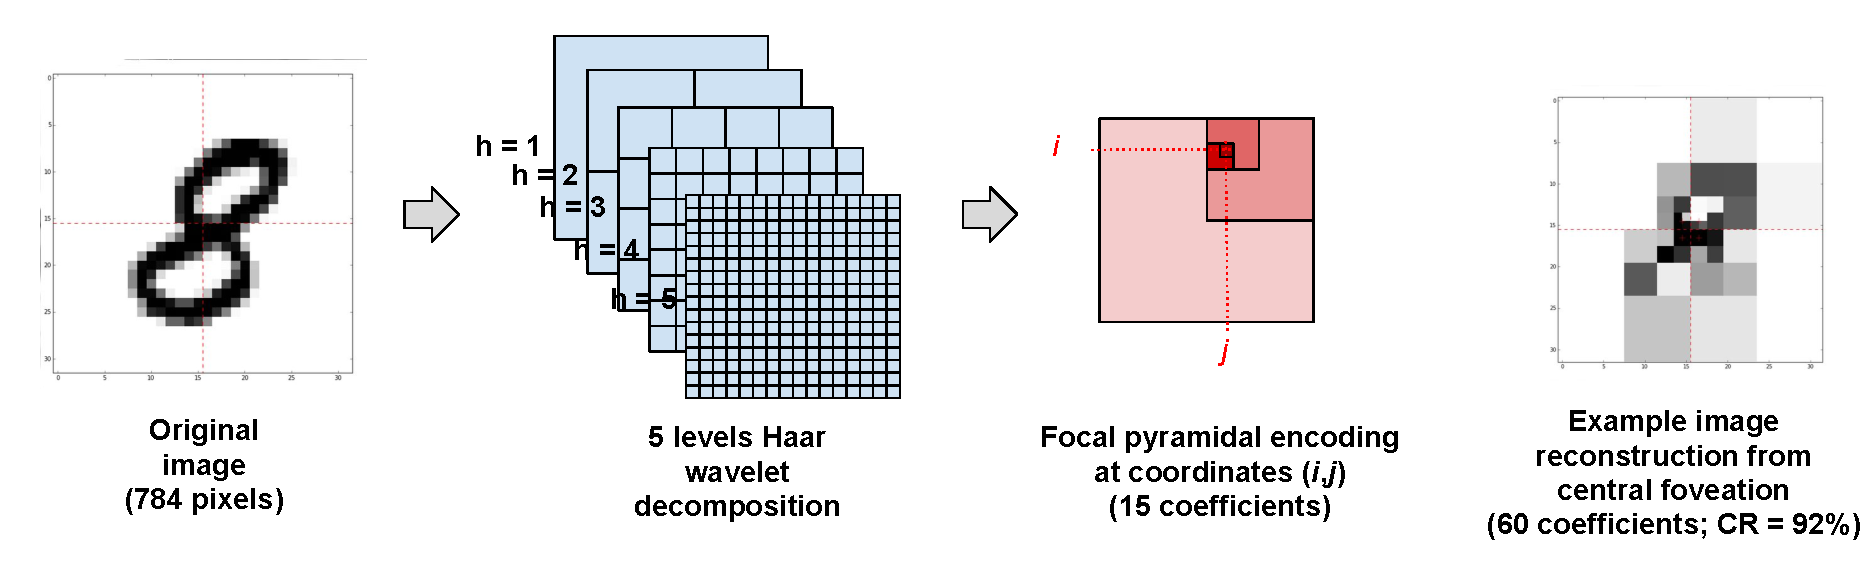
\includegraphics[width = \linewidth]{img/ICLR-foveated-model.pdf} 
	}
	
	\caption{\textbf{a}--\textbf{c}. Foveal ``pyramidal'' encoding from image.
		\textbf{d}. Image reconstruction from 60 central coefficients, issuing a 92 \% compression rate.  
		\textbf{e}. Wavelet-based hierarchical CNN encoder.}\label{fig:foveated}
\end{figure}

The baseline vision model we propose relies first on learning local foveated views on images.
%The essential property of foveated images is that they retain high spatial frequency information at the center and keep only low-frequency information at the periphery.  %Foveated image decomposition is rarely proposed in literature for machine learning purposes, at the exception of Simoncelli's group that has developed a framework to process centrally-magnified images in a bio-realistic fashion (see \cite{freeman2011metamers} and \cite{Deza2016piranhas}). 
Consistently with \cite{kortum1996implementation,wang2003foveation}, we restrain here the foveal transformation to its core algorithmic elements, i.e. the local compression of an image according to a particular focus. Our foveal image compression thus rests on a "pyramid" of 2D Haar wavelet coefficients placed at the center of sight. Taking the example of the MNIST database, we first transform the original images according to a 5-levels wavelet decomposition (see figure \ref{fig:foveated}b). We then define a viewpoint $\boldsymbol{u}$ as a set of 3 coordinates $(i,j,h)$, with $i$ the row index, $j$ the column index and $h$ the spatial scale. Each $\boldsymbol{u}$ generates a visual field made of three wavelet coefficients $\boldsymbol{x}_{i,j,h} \in \mathbb{R}^3$, obtained from an horizontal, a vertical and an oblique filter at location $(i,j)$ and scale $h$.  The multiscale visual information $\boldsymbol{x}_{i,j} \in \mathbb{R}^{15}$ available at coordinates $(i,j)$ corresponds to a set of 5 coefficient triplets, namely $\boldsymbol{x}_{i,j}=\{\boldsymbol{x}_{i,j,5}, \boldsymbol{x}_{\lfloor i/2\rfloor,\lfloor j/2\rfloor,4}, \boldsymbol{x}_{\lfloor i/4\rfloor,\lfloor j/4\rfloor,3}, \boldsymbol{x}_{\lfloor i/8\rfloor,\lfloor j/8\rfloor, 2}, \boldsymbol{x}_{\lfloor i/16\rfloor,\lfloor j/16\rfloor, 1}\}$ (see figure \ref{fig:foveated}c), so that each multiscale visual field owns 15 coefficients (which is a radical compression when the 784 pixels of the original image are considered).
Fig. \ref{fig:foveated}d displays a reconstructed image from the 4 central viewpoints at coordinates (7, 7), (7, 8) (8, 7) and (8, 8).

\paragraph{Algorithms}

%Both the encoder and decoder were trained apart for  
%The discriminator and the generator are trained separately in a supervised fashion so that we 
%our different objectives could be compared on solid ground.
The generic sequential scene decoding setup is provided in algorithms \ref{algo:saccade-policy} and \ref{algo:saccade}. A significant algorithmic add-on when compared with formula
(\ref{eq:predictive-policy}) is the use of a \emph{dynamic actions set} : $\mathcal{U}$. At each turn, the new selected action $\tilde{u}$ is drawn off from $\mathcal{U}$, so that the next choice is made over fresh directions that have not yet been explored. This implements the inhibition of return principle stated in \cite{itti2001computational}. A second algorithmic aspect is the use of a threshold $H_\text{ref}$ to stop the evidence accumulation process when enough evidence has been gathered. This threshold is a free parameter of the algorithm that sets whether we privilege a conservative (tight) or optimistic (loose) threshold. The stopping criterion needs to be optimized to arbitrate between resource saving and coding accuracy. 


\begin{algorithm}[t]
	\caption{Prediction-Based Policy}\label{algo:saccade-policy}
	\begin{algorithmic}
		\REQUIRE  $p$ (decoder), $q$ (encoder), $\rho$ (prior), $A$ (objective), $\mathcal{U}$ (actions set)
		%\STATE predict $z \sim \rho$
		\FOR{$\boldsymbol{z},\boldsymbol{u} \in \mathcal{Z,U}$}
		\STATE sample: $\tilde{\boldsymbol{x}}_{z,u} \sim p(\boldsymbol{x}|\boldsymbol{z},\boldsymbol{u})$
		\STATE $r(\boldsymbol{z},\boldsymbol{u}) \leftarrow A(\boldsymbol{z},\boldsymbol{u},\tilde{\boldsymbol{x}}_{z,u},q,\rho)$ 
		\ENDFOR
		\RETURN $\tilde{\boldsymbol{u}} = \underset{\boldsymbol{u} \in \mathcal{U}}{\text{argmax }} \langle\rho, r(:,\boldsymbol{u})\rangle$
	\end{algorithmic}
\end{algorithm}

\begin{algorithm}[t]
	\caption{Scene Exploration}\label{algo:saccade}
	\begin{algorithmic}
		\REQUIRE  $p$ (decoder), $q$ (encoder), $\rho_0$ (initial prior), $A$ (objective), $\mathcal{U}$ (actions set)
		\STATE $\rho \leftarrow \rho_0$ 
		\WHILE {$H(\rho) > H_\text{ref}$}
		\STATE choose: $\tilde{\boldsymbol{u}} \leftarrow \text{Prediction-Based Policy}(p, q, \rho, A, \mathcal{U})$
		\STATE read: $\boldsymbol{x}_{\tilde{u}}$
		\STATE update: $\forall z, \text{odd}[z] \leftarrow \log q(z|\boldsymbol{x}_{\tilde{u}},\tilde{u};\rho)$ 
		\STATE $\rho \leftarrow \text{softmax} (\text{odd})$ \COMMENT{\emph{the posterior becomes the prior of the next turn}}
		\STATE $\mathcal{U} \leftarrow \mathcal{U} \setminus \{\tilde{u}\}$ 
		\ENDWHILE
		%		\RETURN $\rho$
	\end{algorithmic}
\end{algorithm}

The actual saccade exploration algorithm moreover adapts algorithm \ref{algo:saccade} the following way. The process starts from a loose assumption based on reading the root wavelet coefficient of the image, from which an initial guess $\rho_0$ is formed. Then, each follow-up saccade is calculated on the basis of the final coordinates $(i,j) \in [0,..,15]^2$, so that the posterior calculation is based on several coefficient triplets. After selecting $(i,j)$, all the corresponding coordinates $(h,i,j)$ are discarded from $\mathcal{U}$ and can not be reused for upcoming posterior estimation (for the final posterior estimate may be consistent with a uniform scan over the wavelet coefficients). 

\begin{figure}[b!]
	\centerline{
		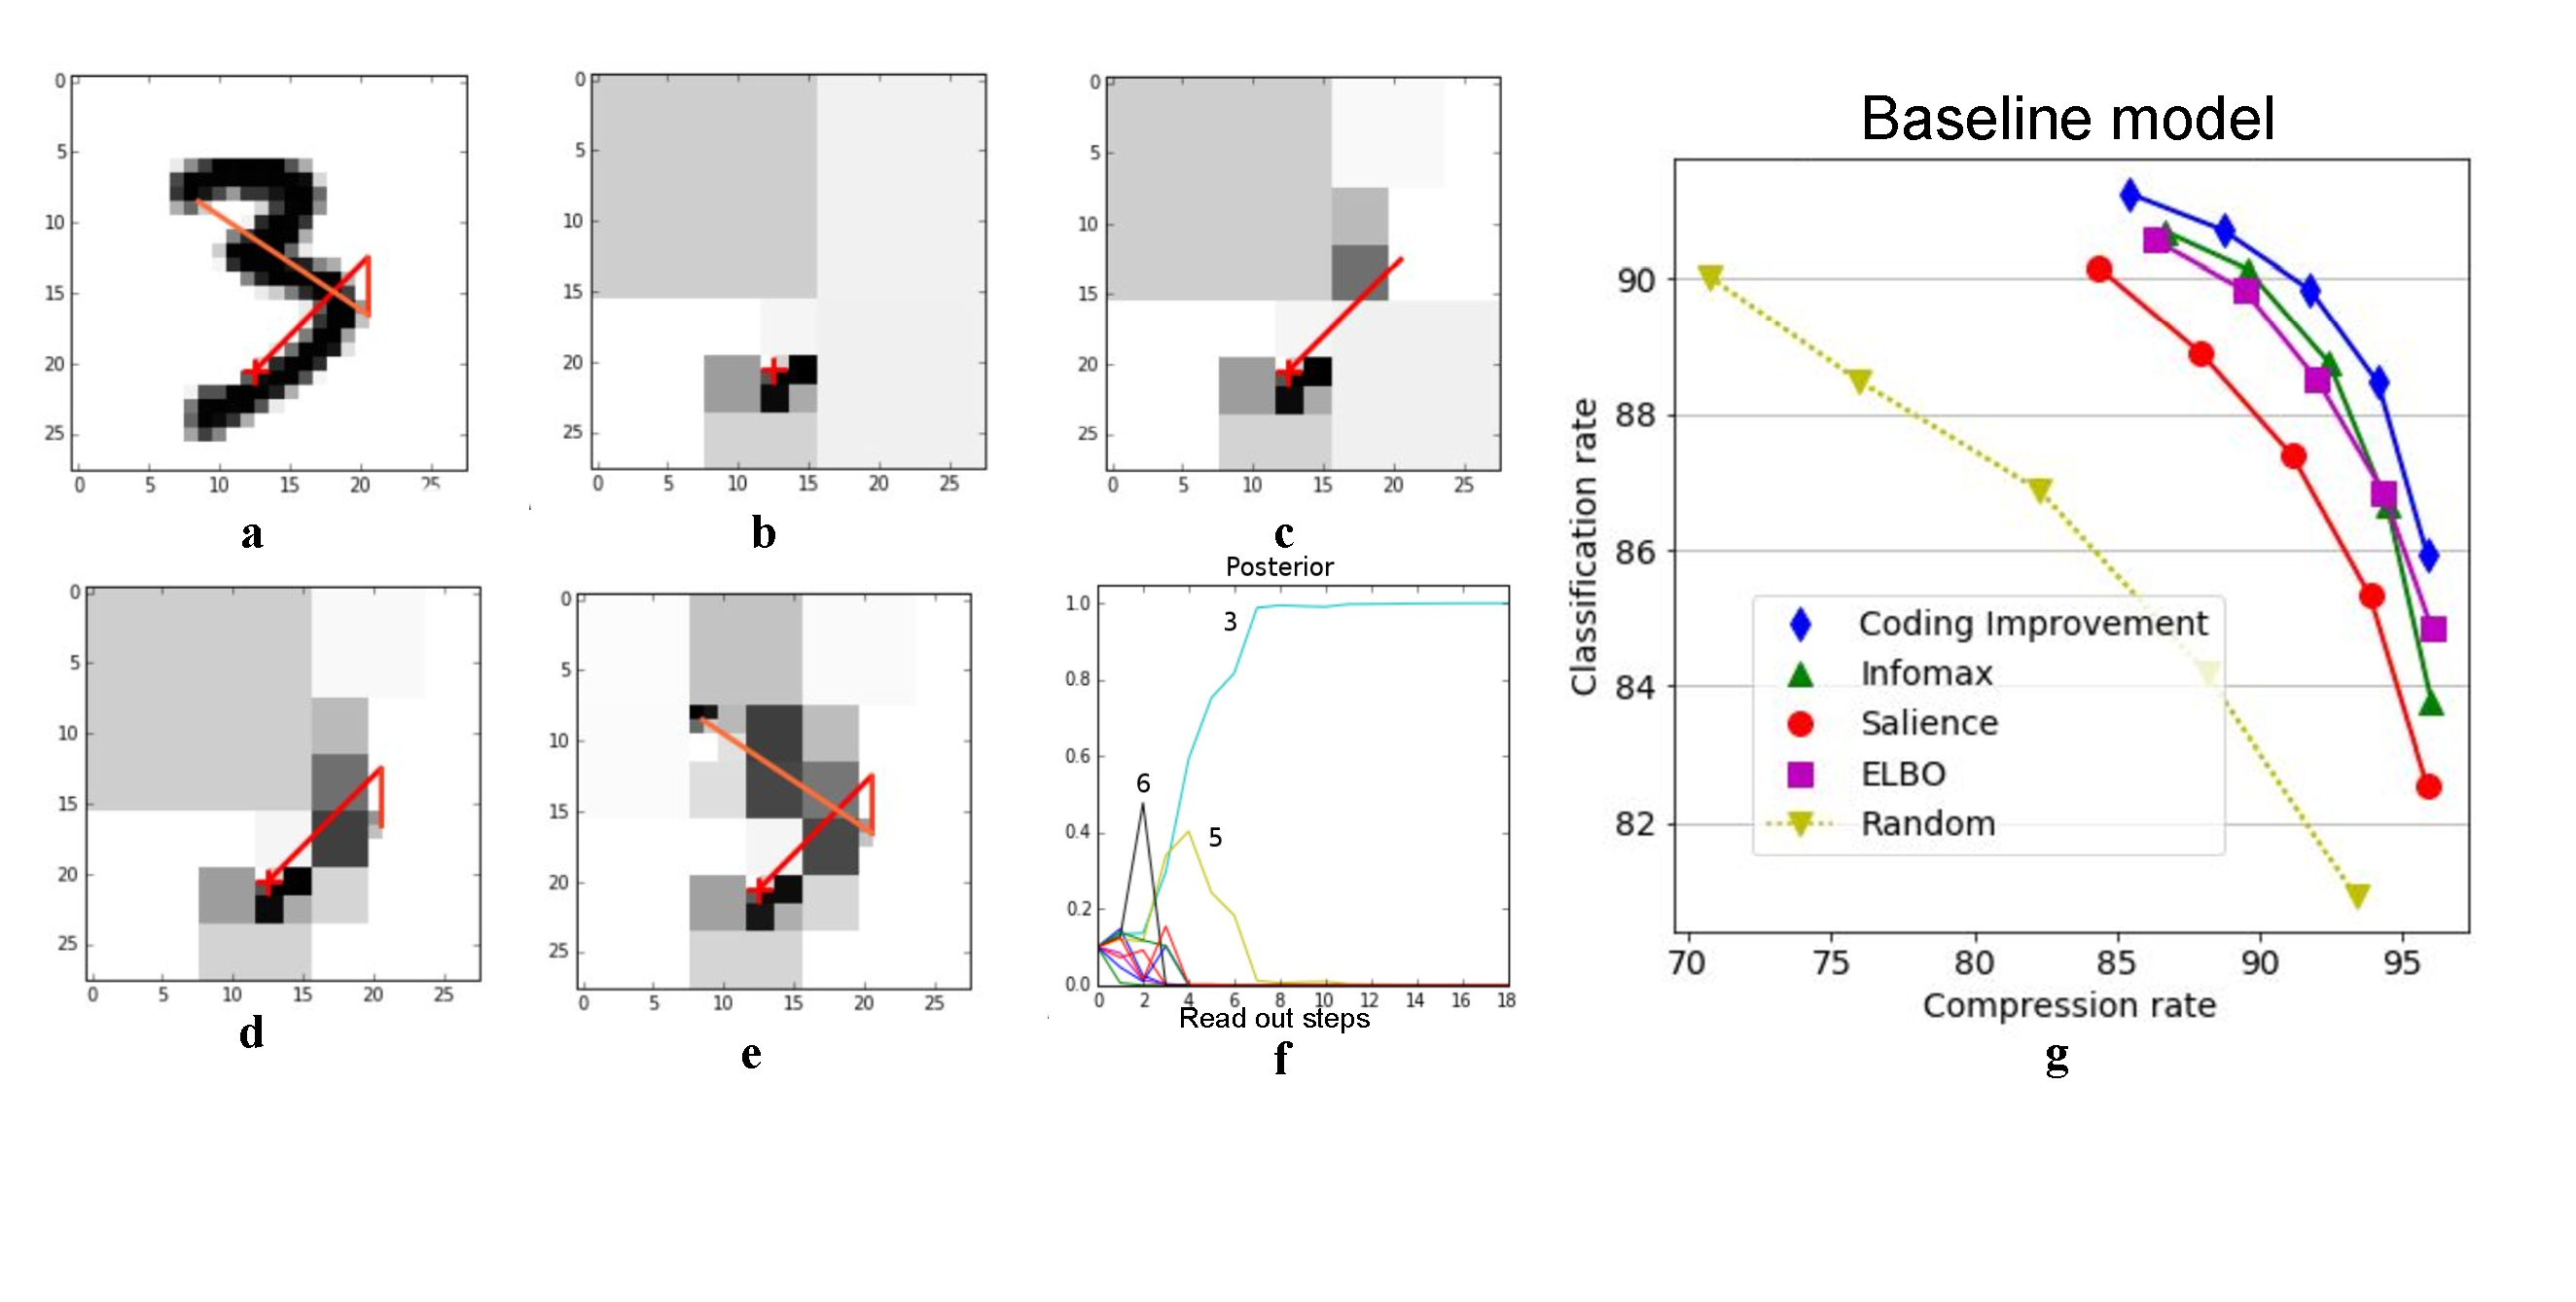
\includegraphics[width=\linewidth]{img/NIPS-saccade.pdf}}
	\vspace{-.2cm}
	\caption{\textbf{Scene exploration through saccades in the foveated vision model}. \textbf{a}. Saccades trajectory over the original image (initial gaze orientation indicated with a red "plus"). \textbf{b--e}. Progressive image reconstruction over the course of saccades, with \textbf{b}: 5 coefficients triplets + root coefficient (initial gaze orientation), \textbf{c}: 9 coefficients triplets + root coefficient (first saccade), \textbf{d}: 13 coefficients triplets + root coefficient (second saccade), \textbf{e}: 17 coefficients triplets + root coefficient (third saccade) \textbf{f}. Posterior update in function of the number of read-out steps (noting that step 1 stems for the root coefficient and the next steps stem for 3 Haar wavelet coefficients read-out), with one color per category (the numbers over the lines provide the competing labels) \textbf{g}.  Classification rate measured on the test set in function of the decoding compression rate, for different objective functions. The stopping criterion varies from $H_\text{ref}=10^{-5}$ up to  $H_\text{ref}=10^{-1}$ (from left to right).}\label{fig:foveated-saccades}
\end{figure}

\paragraph{Baseline generative model and decoding compression}
A generative model is learned for each $\boldsymbol{u} = (i,j,h)$ (making a total of 266 data models) over the 55,000 examples of the MNIST training set. For each category $\boldsymbol{z}$ and each gaze orientation $\boldsymbol{u}$, a generative model is built over parameter set $\Theta_{\boldsymbol{z},\boldsymbol{u}} = (\rho_{\boldsymbol{z},\boldsymbol{u}}, \boldsymbol{\mu}_{\boldsymbol{z},\boldsymbol{u}}, \boldsymbol{\Sigma}_{\boldsymbol{z},\boldsymbol{u}})$, so that 
\begin{align}
\forall \boldsymbol{z},\boldsymbol{u}, \tilde{\boldsymbol{x}}_{\boldsymbol{z},\boldsymbol{u}} \sim \mathcal{B}(\rho_{\boldsymbol{z},\boldsymbol{u}}) \times \mathcal{N}(\boldsymbol{\mu}_{\boldsymbol{z},\boldsymbol{u}}, \boldsymbol{\Sigma}_{\boldsymbol{z},\boldsymbol{u}})\label{eq:bernouilli-gated}
\end{align} 
with $\mathcal{B}$ a Bernouilli distribution and $\mathcal{N}$ a multivariate Gaussian. The role of the Bernouilli is to ``gate'' the multivariate Gaussian model in the high frequencies, where digit deformations is reflected in an alternating presence or absence of pixels for high level coefficients and at the periphery, allowing to discard the ``white'' triplets from the Gaussian moments calculation. Each resulting generative model $p(X|Z,\boldsymbol{u})$ is a mixture of Bernouilli-gated Gaussians over the 10 MNIST labels. On the encoding side, the posterior is explicitly calculated using Bayes rule, i.e. $q(Z|\boldsymbol{x},\boldsymbol{u}) = \text{softmax} \log p(\boldsymbol{x}|Z,\boldsymbol{u})$, issuing about 92\% recognition rate on the MNIST test set when combining the 266 log likelihoods of each wavelet triplet of the full images with (\ref{eq:accum}), a typical recognition rate for shallow models.

The example of an ``Infomax''-based sequential scene decoding is presented in figure \ref{fig:foveated-saccades}\textbf{a}--\textbf{f} for one MNIST sample using algorithm \ref{algo:saccade}.
The original image is presented in fig~\ref{fig:foveated-saccades}\textbf{a} with on overlay a four ``saccades'' trajectory over the image. The corresponding decoding process is illustrated in figs~\ref{fig:foveated-saccades}\textbf{b}--\textbf{e}, giving the reconstructed pixels from  coefficients read-out at successive steps of the decoding process.
%The state of the recognition process after one saccade is shown on fig. \ref{fig:foveated-saccades}\textbf{b}. The next saccade (fig. \ref{fig:foveated-saccades}\textbf{c})  heads toward a region of the image that is expected to help confirm the guess. The continuing saccade (fig. \ref{fig:foveated-saccades}\textbf{d}) makes a close-by inspection and the final saccade (fig. \ref{fig:foveated-saccades}\textbf{e}) allows to reach the posterior entropy threshold, set at $H_\text{ref} = 1e^{-4}$ here. Fig. \ref{fig:foveated-saccades}\textbf{f} shows the posteriors update of different labels over the decoding sequence and fig. \ref{fig:foveated-saccades}\textbf{g} gives the posterior entropy update according to the coefficients triplets actually read. 
Note that several coefficient triplets are read at each end-effector position ($i,j$) (see fig. \ref{fig:foveated}c). There is for instance a total of 5 triplets read out at the initial gaze orientation (\textbf{b}), and then 4 triplets read-out for each continuing saccade. 
Last, the \emph{decoding compression rate} is defined as the proportion of wavelet coefficients that are bypassed for reaching decision. In the considered example, a total of 18 coefficient triplets is  actually read-out, representing about 7\% of the total 256 coefficient triplets, issuing a 93\% decoding compression rate. 

Fig.~\ref{fig:foveated-saccades}\textbf{g} shows the classification rate and the decoding compression rate  obtained in the test set for different objective functions and $H_\text{ref} \in \{10^{-1}, 10^{-2}, 10^{-3}, 10^{-4}, 10^{-5}\}$. The objectives are also compared with a random baseline policy. The classification rates monotonically increase with an \emph{decreasing} recognition threshold. Considering 92\% as the upper bound here, a near optimal recognition rate is obtained  at $H_\text{ref}=1O^{-5}$ for the CI objective. Though all objectives functions show a consistent increase of the classification rate with decreasing $H_\text{ref}$, the compression improvement objective clearly overtakes the others ones. The Infomax and the ELBO behave in a close-by fashion, and then the Salience objective seems unfitted to the task. 
The compression rates are generally good, with a close to optimal classification obtained at 85\% compression. It needs to be noticed that still a correct 90\% classification rate can be obtained with random exploration at around 70\% compression rate, reflecting a strong redundancy in the original dataset.  

%The model provides apparently realistic saccades, for they cover the full range of the image and tend to point over regions that contain class-characteristic pixels. The image reconstruction after 4 saccades allows to visually recognize a "fuzzy" three, while it would not necessarily be the case if the saccades were chosen at random.
%The observed trajectory illustrates the \emph{guess confirmation} logic that is behind the active vision framework. Every saccade heads toward a region that is supposed to confirm the current hypothesis. This confirmation bias appears counter-intuitive at first sight, for some would expect the eye to head toward places that may \emph{disprove} the assumption (to challenge the current hypothesis). This is actually not the case for the class-confirming regions are more scarce than the class-disproving regions, so that heading toward a class-confirming region may bring more information in the case it would, by surprise, invalidate the initial assumption.

%{\color{green} With a final posterior approaching $1 - 1e^{-5}$, the model is actually overconfident in its own predictions which introduces a confirmation bias that may harm the final recognition rate. This is not the case in our setup (see next section for quantitative accuracy estimate), but one can not exclude the process to be overconfident at a local minimum. It must be noticed however that the confirmation bias is a more general feature of the active inference framework that should be specifically addressed (with a $T$-horizon forward planning at exponential cost and/or reward-based policy learning -- see \cite{butko2010infomax}). For there is no free lunch, it corresponds to the "price to pay" for reducing the observation range of the image at the risk of potentially neglecting critical covert information. }

\begin{figure}
	\centerline{
		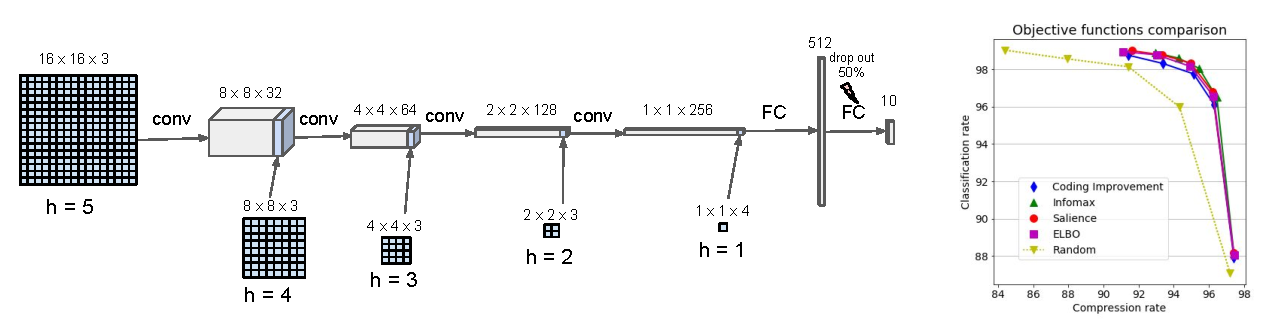
\includegraphics[width = \linewidth]{img/NIPS-convolutional.pdf} 
	}
	\vspace{-.2cm}
	\caption{\textbf{Hierarchical Convolutional Neural Network for Scene Decoding}. (Left) The CNN computational graph reflects the input hierarchical organization. (Right) Objective functions comparison on the CNN model.}\label{fig:CNN}
\end{figure}

\paragraph{Posterior update in Convolutional Neural Networks}
A convolutional neural network was designed in order to provide a more effective encoding and facilitate comparison with state-of-the-art classifiers (see fig.~\ref{fig:CNN}). 
It is made of five convolution layers having each a distinct input corresponding to the five hierarchical levels of the wavelet decomposition. 
The CNN is biasless, uses a (2,2) stride for the convolutions \emph{without max-pooling}, maximizing \emph{neighbour independence} in the convolutional computational track.
The training data was compressed at random by discarding wavelet coefficient triplets, with a varying compression rate. Rectified Linear Units are used in all layers, except for the final layer owning linear units. The network was trained during about $10^6$ epochs with Tensorflow on a laptop. Without specific parameter tuning, the network attained a 99\% recognition rate on the test set with non-compressed wavelet transformed inputs. 

The cross-entropy loss used in training makes the network output is expected to approach the data log-likelihood, and this is how it is exploited further on. For decoding a scene, the input layers are initialized a zero  and progressively filled with new wavelet coefficients, implementing the posterior update \emph{from the data}. There is thus no recurrence, sequential accumulation or memory implemented in the network. The output is driven by adding supplementary data at the input only, complementing the data that was read out at the previous decoding steps. 
Following algorithm \ref{algo:saccade} with the CNN as the encoder, the decoding efficacy is shown for different objective functions on the right-hand side of fig.\ref{fig:CNN}. A clear decoding improvement is obtained, with higher classification rates with less signal, attaining about 98,8\% correct classification with less than 8\% of the original image. Still, the general good performances of the decoder blurs the differences between the different policies. All objectives appear here equally good at effectively decoding the scene. 

\paragraph{Faulty model and failure robustness}
The predictive policies are very dependent on the generative models and thus sensible to model flaws. Resistance to model flaws is thus a property that should be prioritized when acting in unknown or coarsely modeled environments, or in the course of learning. In contrast with CNN-based optimal decoding, we designed a failed probabilistic model by simply setting $\rho_{u,z} = 1$ in eq.~(\ref{eq:bernouilli-gated}).  This tends to overestimate the signal strength at high frequencies, predicting a dense signal in effectively sparse regions. Classification accuracies are presented on fig.~\ref{fig:failed}\textbf{a} for the different objective functions considered here. In complement to the Compression Improvement (eq.~\ref{eq:CI}), the two variants referred as the Local Consistency (eq.~\ref{eq:LC}) and the Posterior Consistency (eq.~\ref{eq:PC}) are also considered. The faulty model allows here to nicely separate the different objectives with regards to their optimistic vs. conservative flavor. While the CI remains on average equivalent to a random sampling, its conservative and optimistic variants respectively do better and worst than random exploration. The ELBO and the Saliency objectives, as expected, amplify this effect with a strong robustness to model flaws for the ELBO objective and, at reverse, a dramatic sensitivity  to model flaws for the 	Saliency objective. The Infomax also falls here in the optimistic category for its blindness to sequential consistency makes it update its posterior the wrong way.

\begin{figure}
	\centerline{
		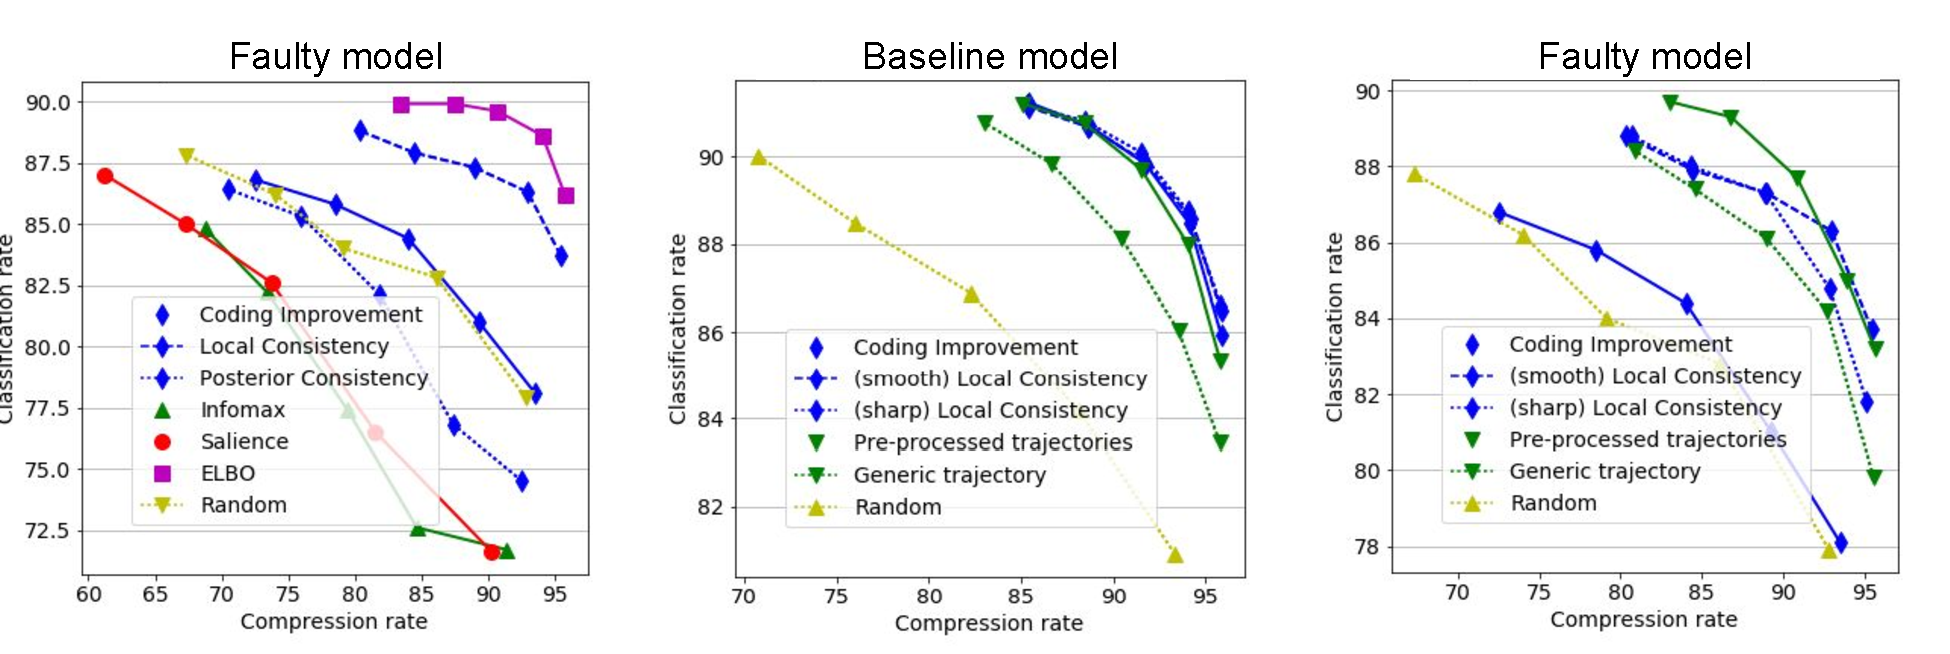
\includegraphics[width = \linewidth]{img/NIPS-faulty.pdf} 
	}
	\vspace{-.2cm}
	\caption{\textbf{Method comparisons}. \textbf{a}. Classification rates comparison in a faulty model (see text). \textbf{b}. Simplified computational schemes compared on the baseline shallow ``Bernoulli gated'' multivariate model. \textbf{c}. Simplified computational schemes compared on the faulty model.}\label{fig:failed}
\end{figure}


\paragraph{Scaling up CI computation}
The scaling of the model needs to be addressed when large control spaces are considered. The predictive policy relies on a mixed encoding setup that implies to consider all $\boldsymbol{u}$'s and all $\boldsymbol{z}$'s in the prediction, which scales like $O(|\mathcal{U}|\times|\mathcal{Z}|^2)$ when the predicted posterior is needed in the objective calculation, which is the case for the Infomax, the Saliency, the CI and the Posterior Consistency (algorithm \ref{algo:saccade-policy}), and $O(|\mathcal{U}|\times|\mathcal{Z}|)$ in the Local Consistency and the ELBO case for they bypass the posterior calculation. A quadratic cost may still be considered too heavy in real-case applications, implying to consider cheaper setups. A first simplification, referred as the ``sharp'' Local Consistency in  fig.~\ref{fig:failed}\textbf{b}, only samples a single $\boldsymbol{z}$ from $q^{(n-1)}$, which makes the predictive policy scale like $O(|\mathcal{U}|)$. An additional simplification can be obtained when considering the Local Consistency objective alone (eq.~\ref{eq:LC}), for it is, on contrary to all other objectives, independent of the context $q^{(n-1)}$. For a given model, all the predictive log posteriors $\log p(\boldsymbol{z}|\hat{\boldsymbol{x}}_{z,u}, \boldsymbol{u})$ can be pre-processed using the \emph{mode} of the predicted visual field $\hat{\boldsymbol{x}}_{z,u} = \underset{\boldsymbol{x}}{\text{ argmax }} p(\boldsymbol{x}|\boldsymbol{z}, \boldsymbol{u})$ as a sample, allowing, for each assumption $\boldsymbol{z}$, to \emph{pre-process} a class-specific visual exploration strategy that, given an assumption $\hat{z} = \underset{\boldsymbol{\boldsymbol{z}}}{\text{ argmax }} q^{(n)}(\boldsymbol{z})$, defines a log-posterior descending order over the $\boldsymbol{u}'s$. It is then possible to pre-process and store $|\mathcal{Z}|$ saccade trajectories of size $|\mathcal{U}|$ in a database, with a $O(|\mathcal{U}|\times|\mathcal{Z}|)$ memory load but only $\simeq O(1)$ readout computational cost. In practice, the viewpoint selected at step $n$ depends on the current guess $\hat{z}$, with on-the-fly trajectory switch if the guess is revised across the course of saccades. This strategy is referred a the \emph{pre-processed trajectories} in figs~\ref{fig:failed}\textbf{b} and \ref{fig:failed}\textbf{c}.
For comparison, a \emph{generic} trajectory was also computed using $\bar{\text{CI}}(\boldsymbol{u})
= \mathbb{E}_{\boldsymbol{z} \sim p(Z), \boldsymbol{x} \sim p(X|\boldsymbol{z}, \boldsymbol{u})}\left[ \log p(\boldsymbol{z}|\boldsymbol{x}, \boldsymbol{u})\right]$ with a uniform prior over the $\boldsymbol{z}'s$.  
It is referred a the \emph{generic trajectory} in figs~\ref{fig:failed}\textbf{b} and \ref{fig:failed}\textbf{c}.

The different simplification strategies are compared in figs~\ref{fig:failed}\textbf{b} and \ref{fig:failed}\textbf{c} over the baseline and the faulty model. Both the sharp Local Consistency and the pre-processed trajectories are shown consistent with the CI objective on fig.~\ref{fig:failed}\textbf{b}, despite their considerably lower computational cost, while the generic trajectory strategy appears less relevant. Interestingly, those computational simplifications also remain effective when robustness to model flaws is considered (fig.~\ref{fig:failed}\textbf{c}). 
Both the sharp Local Consistency and the pre-processed trajectories allow to reach both robustness and effective classification rates at lower cost.

\section{Conclusion}
A generic fovea-based scene decoding setup was presented which, accordingly with \cite{najemnik2005optimal}, rests on a predictive decoding accuracy to choose action. A variational approach to scene encoding is adopted, which, accordingly with \cite{friston2012perceptions}, optimizes the data reconstruction cost by picking new sensory samples through action. In our case, the visual field is interpreted under a \emph{mixed encoding} setup for the visual data is both generated by the viewpoint and the scene constituents. 
This allows to unify the many objective functions proposed in the literature under a single master objective referred as the Compression Improvement in \cite{schmidhuber2007simple}, that is shown to provide a consistent interpretation for most of the objective functions used in perception-driven control. Two variants of the CI objective are proposed, using either the pre-sample or the post-sample posterior in the approximation. In the pre-sample case, it is said the Local Consistency objective and shown to underestimate the actual Information Gain. Following the LC objective is thus expected to lower the risk of failed interpretation in the case of failed predictions. Using the Free Energy \cite{friston2015active} as a loss (instead of the LC) is moreover expected to \emph{bias} the action selection in an even more conservative way. 
Conversely, the Posterior Consistency objective (PC) is shown to \emph{overestimate} the actual Information Gain. Following the PC objective is thus expected to increase the risk of failed interpretation in the case of failed predictions. 
Using the Saliency objective \cite{itti2005bayesian} instead of the PC is moreover expected to \emph{bias} the action selection in an even more optimistic way, subsequently increasing the failed scene interpretation risk.

The presented numerical experiments thus highlight different aspects of the setup. 
A first and principal result is that state-of-the-art recognition rate can be obtained with sequential fovea-based computation using less than 10\% of the original signal. This strong input compression is made possible for the visual data owns lot of redundancies that are not used at their best in computer vision, doing useless computations over large parts of the visual scene. The general good results obtained in that case reflect the advantage of mixing a predictive controller with accurate state-of-the-art predictors, here a deep neural network. 

A second result is the sub-optimality of many classical objective function widely used in literature, like the ``Infomax'' \cite{butko2010infomax} and the ``Salience'' objectives \cite{itti2005bayesian} in the scene decoding setup. Their sub-optimality is not manifest with finely-tuned generative models, but becomes patent when a coarse of faulty model is used.
This may appear counter-intuitive at first sight for the Infomax objective is vastly dominant in predictive control \cite{najemnik2009simple}, while the Salience objective provides among the best predictions for human fixation zones \cite{itti2005bayesian}. The negative performances of the Salience objective in predictive control may however be attenuated when learning is considered. Heading toward inconsistently modeled places is indeed a sensible behaviour when the model is to be updated. This entails maximizing predictions errors, which is a decent principle long considered in sparse reinforcement learning \cite{schmidhuber1991curious,oudeyer2008can,mohamed2015variational}. The main difference lies in considering model-based predictive rewards, as we do here, versus model-free post-hoc rewards. In the second case, a n \emph{observed} inconsistency reflects a model flaw that needs to be adressed, while in the first case, it only reflects a predictive inconsistency, that is part of the model, favoring oblivious rather than memory-consistent scene interpretation. This trade-off between predictive versus post-hoc reward reflects more generally a profound contradiction between exploiting at best the current knowledge and past observations versus challenging the current interpretation to leverage conflicting facts, a variant of the exploration/exploitation trade-off. 

Last, a notorious flaw of the predictive setup is its large complexity when large action sets are considered. Real-world predictive control is in need for computationally-effective models, here attainable with the Local Consistency objective (LC), that, though maximizing the Information Gain in approximation,  is shown to provide both a good robustness to model flaws and ways toward cheap and scalable predictive policies.  


\bibliographystyle{apalike}
\bibliography{biblio}

\end{document}